% ------------------------------------------------------------------------ %
% !TEX encoding = UTF-8 Unicode
% !TEX TS-program = pdflatex
% !TEX root = ../Tesi.tex
% !TeX spellcheck = en_US
% ------------------------------------------------------------------------ %
%
% ------------------------------------------------------------------------ %
% 	CONCLUSIONI
% ------------------------------------------------------------------------ %
%
\chapter{Case Study}
%
\label{cap:proofofconcept}
%
% ------------------------------------------------------------------------%
In this chapter I will describe the real implementation of the system, which is the real solution of the problem faced by this thesis work: how it is possible to extend a mobile operating system, in this case Android, with distributed OS functionalities.\\
This chapter is mainly composed of three parts: the first one is a generic information
section in which the proof of concept is explained in terms of technologies
used, requirements to meet, goals and various technicalities. The second one
is the report of the implementation and development of the application, with
choices and descriptions of what has been done. The third part is a working demo of the
just described system, with live working test cases. It contains screenshots of the
application while it is running and a complete description to explain each case
step by step.
\section{Conception}
As already specified in the previous chapter my system has been implemented as a standard Android application, which can be installed on any Android device starting from the API level 19, Android 4.4 KitKat. The final APK package contains all the files needed for the system installation, and, once installed, the application performs the extension of the Android OS giving to it distributed functionalities. I will use the complete API described in \ref{API} to implement a background working middleware to distribute implicit intent in a LAN to any Android device with the service installed. In this way every time one of the device, having the \textit{Liquid Android APK}
installed, triggers an implicit intent, my application could intercept and send it to any other device to be resolved and executed. The idea of this prototype is to prove that what I have stated, providing the theoretical solution, can work with a real configuration of Android devices in any LAN. Doing this, the thesis work is somehow \textit{"proved"}: my communication language, defined with a JSON file, is concretely usable and working, not to worry the users about the kind of implicit intent they need to execute in one of the devices in the network. The translation process does not represent an issue for my application, because I have developed an automatic intent translator using the correct syntax proposed by me. I will not develop clients for third party systems, even if I stated that it would be possible, especially in Java environments, but I will implement a simple Android application client, generating some standard implicit intent to perform some test with my system.
\subsection{Requirements}
In this small subsection I want to provide a full list of requirements my application must meet. In order to be considered a solution of the given problem, it must fulfill the constrains listed in \ref{problemconstraints} and also comply with functional and non functional requirements.
\subsubsection{Functional Requirements}
Functional requirements are, indeed, the main functionalities the systems must have in order to properly work to perform desired task.\\
The following lists summarize the main features of the system, so as to ensure a quick reference while reading this document:
\begin{itemize}
	\item \textbf{FR1}: listen to implicit intents.\\My application should declare itself, in the android manifest, as a multipurpose application which can be used to resolve, basically, any kind of implicit intents, in order to be selected by the Android OS whenever an intent resolution process is triggered.
	\item \textbf{FR2}: JSON to Intent, and Intent to JSON, conversion.\\ My application must be able to perform the conversion using the JSON syntax i have explained in \ref{syntax}.
	\item \textbf{FR3}: forward implicit intents.\\ My application must be able to forward any of the implicit intent it can listen, to other LAN connected devices with the \textit{Liquid Android APK} installed.
	\item \textbf{FR4}: receive and execute intents.\\ My application must be able to receive in any moment implicit intents, as JSON-Intent object, and then, let the OS resolve and execute them with its standard mechanisms.
\end{itemize}
\subsubsection{Non-Functional Requirements}
Non-functional requirements are important properties that my
system must have in order to guarantee full functionalities. They are not specific
for my problem but, they are general requirements a system needs to be considered complete. It is quite clear how a system can use my language but if it takes 15 minutes to perform a translation or to deliver a message it is completely useless.\\
Non-functional requirements in this way complete my system, they are mainly:
\begin{itemize}
	\item \textit{Portability}: to have my application used by the largest number of users
	possible, so i have made the choice to use Android API level 19, to allow the installation of my system to, more or less, the 84\% of Android devices currently active.
	\item \textit{Stability}: system must be always available, and able to offer all its services. For example I should avoid possible system crashes during the delivery of a message from a device to another. In addition, data must be durable and not lost for any reasons.
	\item \textit{Availability}: the services must be always accessible in time. In case of failures it is possible for the user to manually restart it to be again usable.
	\item \textit{Reliability}: since data are shared among devices, reliability is essential. Users can base their actions on other users’ actions and on the status of the devices. Moreover, I assume that the memory where data are stored is stable.
	\item \textit{Efficiency}: within software development framework, efficiency means
	using as few resources as possible. Thus, the system will provide data
	structures and algorithms aimed to maximize efficiency. I will also try to
	use well known patterns reusing as many pieces of code as possible, taking
	care of avoiding any anti-patterns.
	\item \textit{Extensibility}: my application must provide a design where future updates
	are possible. It will be developed in such a way that the addition of new
	functionalities will not require radical changes to the internal structure and
	data flow.
	\item \textit{Maintainability}: also modifications to a code that already exists have to be
	taken into account. For this reason the code must be easily readable and
	fully commented.
	\item \textit{Security}: Using a networking service security is always required. The fact that
	the system will be available only on LANs is the first step in this direction.
\end{itemize}
\subsection{Used Technologies}
This other subsection is an overview of the tools I have used to develop the
Android application.\\
Android applications are written using Java code and any API level of the Android framework. The \textit{Liquid Android APK} is been developed by using standard Android development tools and libraries without the need to rely on any third party API library. In particular I decided to make these choices.
\begin{itemize}
	\item \textit{Android API level 19}, as already explained several times I want that my system can be installed on the largest number of devices, so it is a compromise between the great innovation introduced starting from this API level, and the number of devices which can execute API level 19 apps.
	\item \textit{Android NSD library}, it is a standard Android library I am using to register, discover and resolve my network service. It is an implementation of Zeroconf and it is compatible with other implementation such as Apple's bonjour.
	\item \textit{Standard Java libraries}, I decided to use only libraries included in standard Java development kit distribution, the most important are :
	\begin{itemize}
		\item \textit{org.json}, used to manage the JSON file, which are the messages exchanged by the devices using my application;
		\item \textit{java.net}, containing the classes which are useful to implement the socket network communication.
	\end{itemize}	
\end{itemize}
Technically, I used an IDE to help in development, in particular AndroidStrudio based on IntelliJ IDEA, a
modern solution released by Jet Brains. It contains modern tools to check Java
compile time errors flagging them, and tools to check run time errors with a
complete and verbose stack trace.Finally,
it supports various VCS (Versioning control systems), to push the code inside
repositories and to have a complete overview of commits and forks. I chose Git,
one of the most famous VCS, and GitHub as repository to save my code.
\subsection{Implementation}
I have developed a fully working Android application called \textit{Liquid Android}. I have build the application using the API library i have created and already presented in \ref{API}, so the structure of my code follows exactly the one presented with the \textit{Liquid Android API} UML model, in \figurename~\ref{fig:4.7}. The components and the methods i have used, to create the application, are exactly the one presented in that figure with little modifications and adaptations.
\subsubsection{Code organization}
\begin{figure}[h]
	\centering
	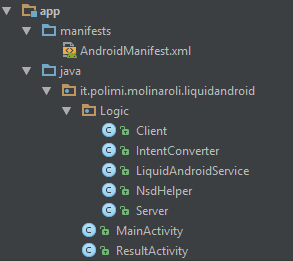
\includegraphics[width=.45\textwidth]{package}
	\caption{Code organization}
	\label{fig:5.1}
\end{figure}
As anticipated, the code is organized following the \textit{MVC} design pattern, so the \textit{controller components} are all contained in the \textit{Logic} package, while the \textit{UI components} are left inside the \textit{Main} package of the application- Other components typical of the Android development framework are left in their standard locations, such as the XML file containing the \textit{application manifest}.

\subsubsection{Implicit Intents to listen}
\lstinputlisting[language=XML , caption=Liquid Android MainActivity Manifest example, label=code:5.1]{Codici/manifest.xml}
In \lstlistingname~\ref{code:5.1} there is part of the manifest, of my application, showing some common intent filters which the \textit{Liquid Android} app can listen to. In figure we can see that is the MainActivity of the application which declare itself capable of managing intents to take a picture, send and email or open a map. By adding any intent filter to the manifest of the application Liquid Android can listen and forward, automatically any kind of Android implicit intent. This snippet of code is the way in which the \text{FR1} is practically implemented.\\\\
In the following section I want to describe my system in action, providing application's screenshots, UML diagrams, working tests and use cases.
\section{Working Demo}
This section is intended to show the reader the \textit{Liquid Android Application} while it is working. After the structure and the implementation of the application were explained it is necessary to show the finished work. As anticipated, my application
is simply a proof of concept of how it is possible to use a group of Android devices, as they were executing a single distributed operating system using well known  Android mechanisms. Users should not worry about substrates, they can control everything with a single and simple standard Android UI.\\
I set up the demo by creating a LAN with a wireless router, and then I installed my application on three smartphones, connected both to Android Studio to debug the applications reading the consoles, and to the wireless LAN. This is only one possible environment configuration for my middleware application, but is enough simple and significant to provide a proof of my work.\\
I developed, also, for testing purposes, a simple client application able to generate standard Android implicit intents, which I will use to perform some live test cases. I called this Android app, \textit{Intent Generator} which has the only feature of create intents and then ask the OS to resolve them. The same result can be obtained using any standard Android app which generates implicit intents and passes them to the OS to be solved.
\subsection{Liquid Android UI}
\begin{figure}[h]
	\centering
	\begin{minipage}{.49\textwidth}\centering
	\subfloat[Main Activity UI\label{subfig-1:main}]{%
		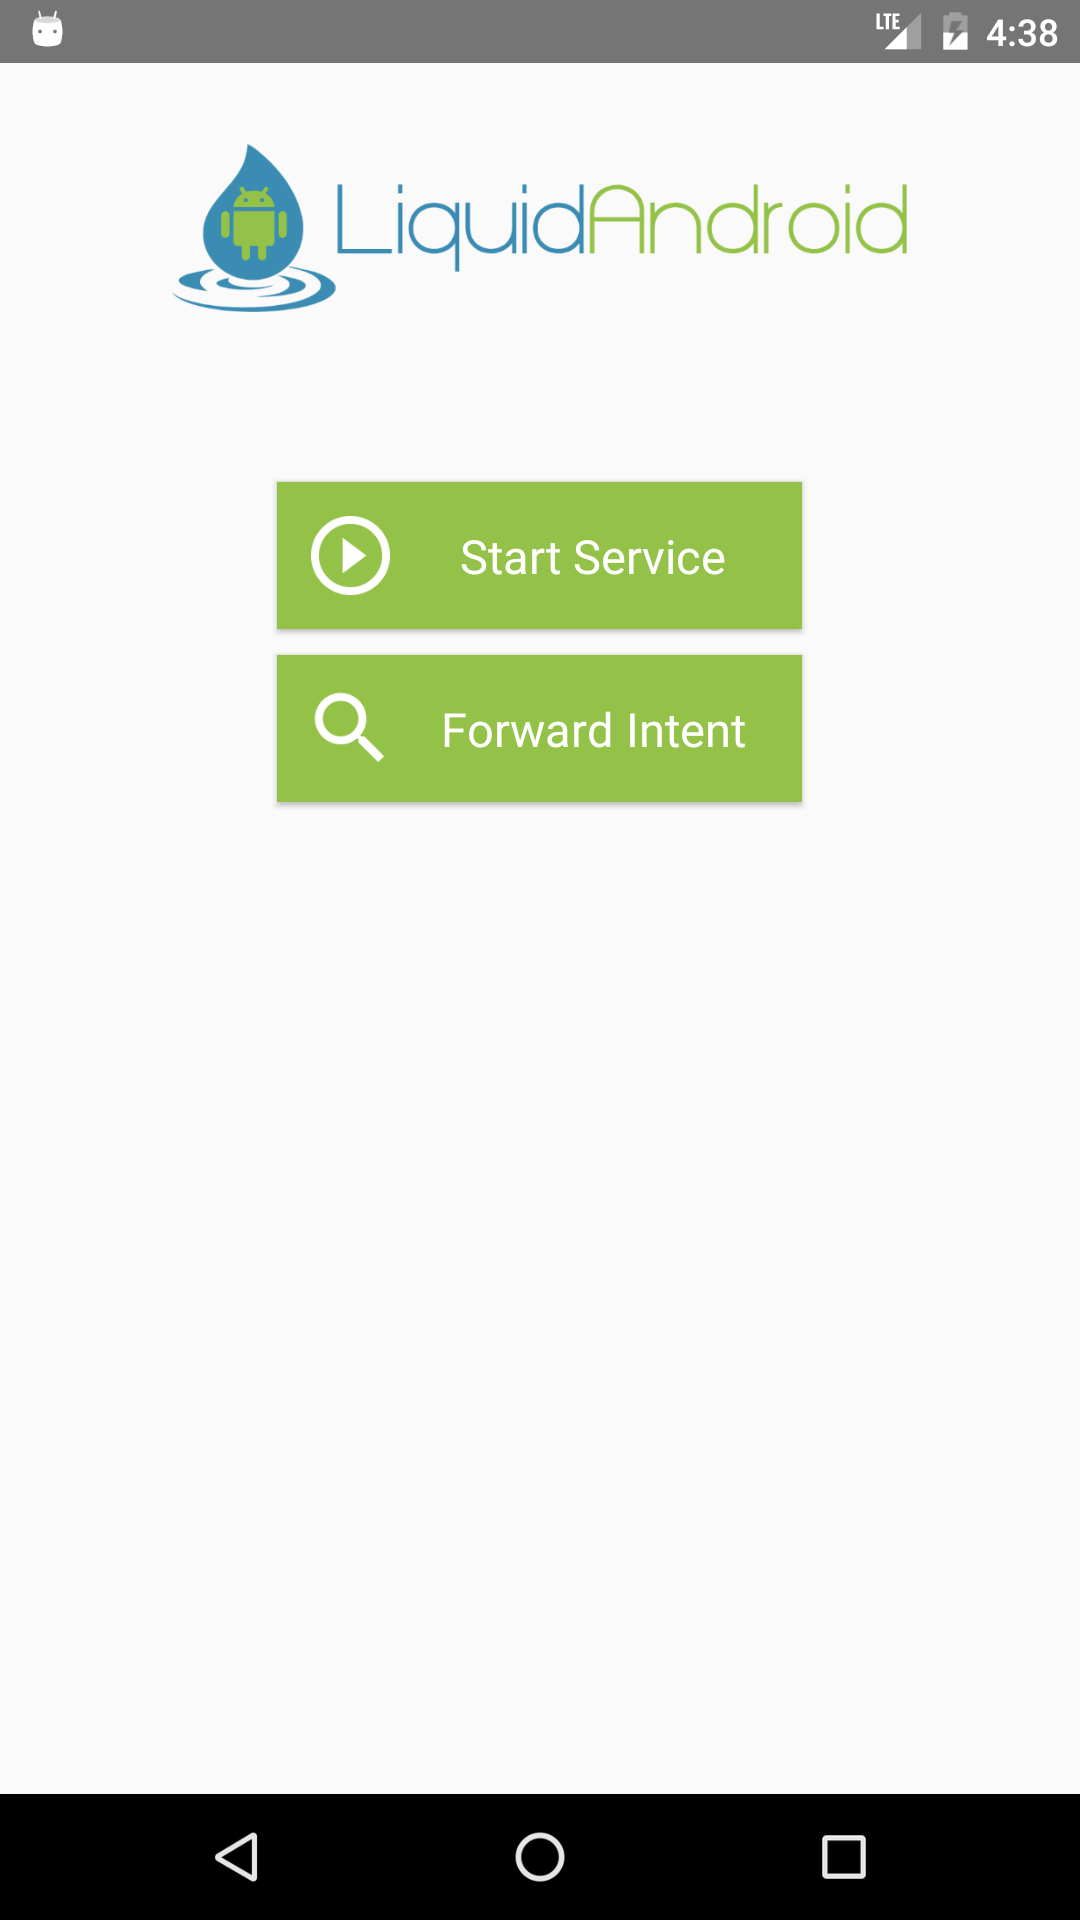
\includegraphics[width=0.75\textwidth]{main}
	}
	\end{minipage}
	\begin{minipage}{.49\textwidth}\centering
	\subfloat[Notification UI\label{subfig-2:notification}]{%
		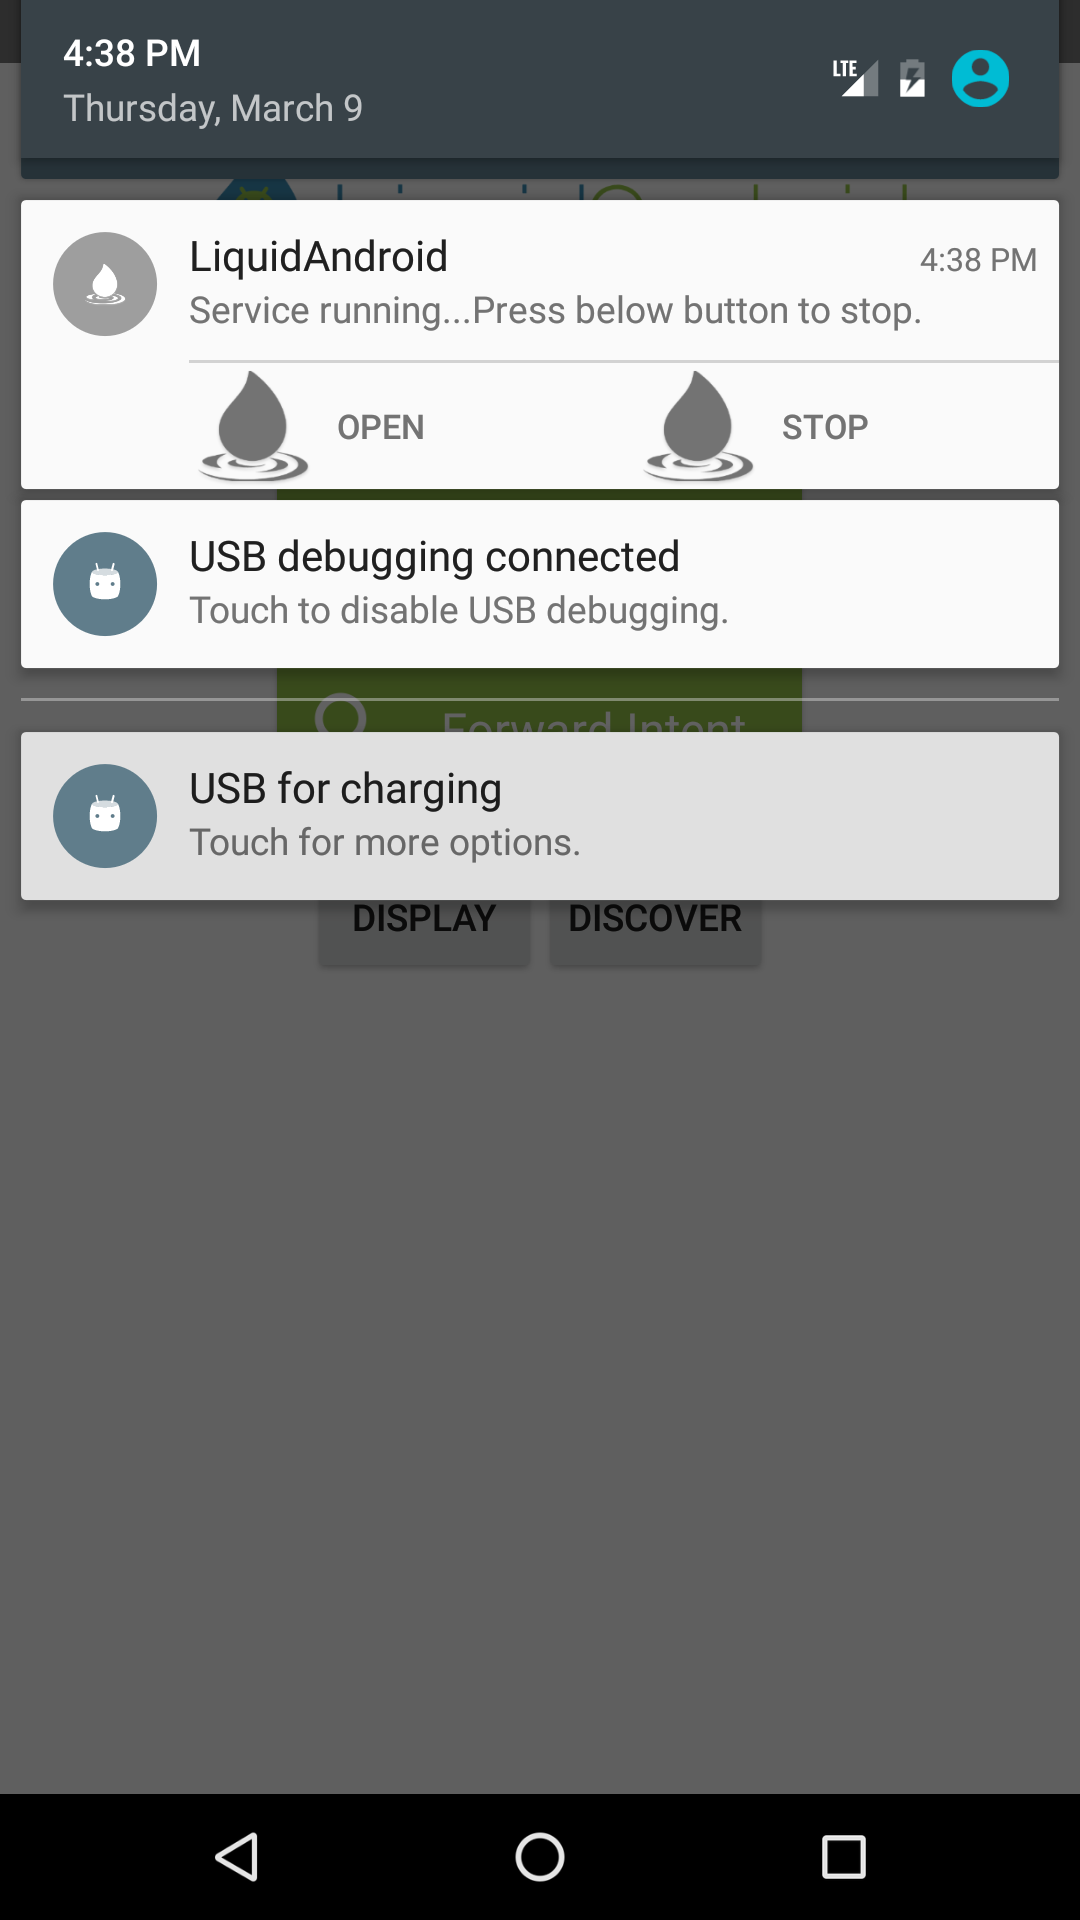
\includegraphics[width=0.75\textwidth]{notification}
	}
	\end{minipage}
	\caption{Main Liquid Android UI components}
	\label{fig:5.2}
\end{figure}

Once installed the Liquid Android application on a compatible device, users can control it by its MainActivity and its \textit{foreground service} notification, when the service is in execution. The \figurename~\ref{fig:5.2} shows the Liquid Android application's main UI components. By clicking the button \textit{Start Service} the middleware executes and the extension of the Android OS is performed by the application. Once clicked the button the server component of the application is up, and the network service is registered in the LAN, moreover the notification showed in \ref{subfig-2:notification} appears in the Android notification area. From that notification, users can control the status of the service, because it can not be removed from the Android notification area until the service is stopped by clicking the stop button, embedded in the notification. The other embedded open button, instead, starts the MainActivity, in \ref{subfig-1:main}, and puts it in foreground.\\
\begin{figure}[h]
	\centering
	\begin{minipage}{.49\textwidth}\centering
		\subfloat[App Chooser Dialog UI\label{subfig-1:intent}]{%
			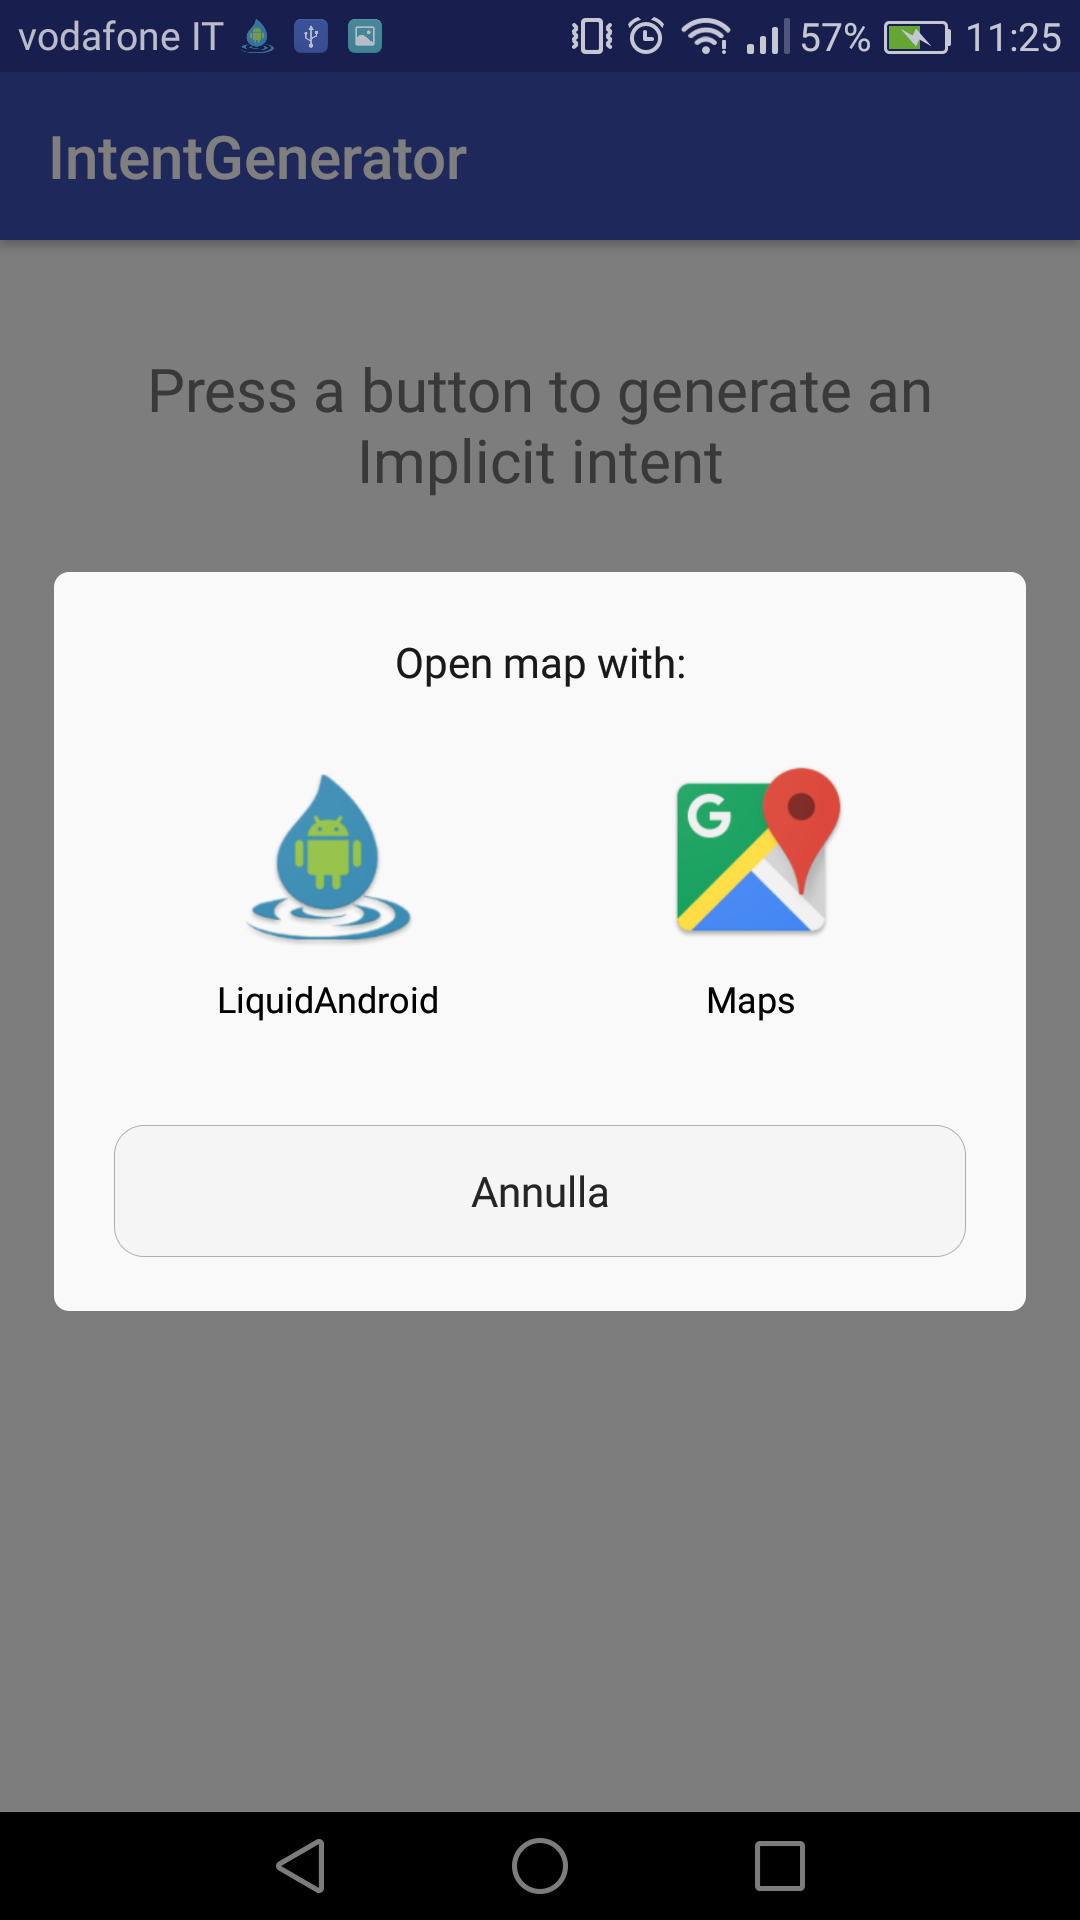
\includegraphics[width=0.75\textwidth]{selector}
		}
	\end{minipage}
	\begin{minipage}{.49\textwidth}\centering
		\subfloat[Forward Dialog UI\label{subfig-2:forward}]{%
			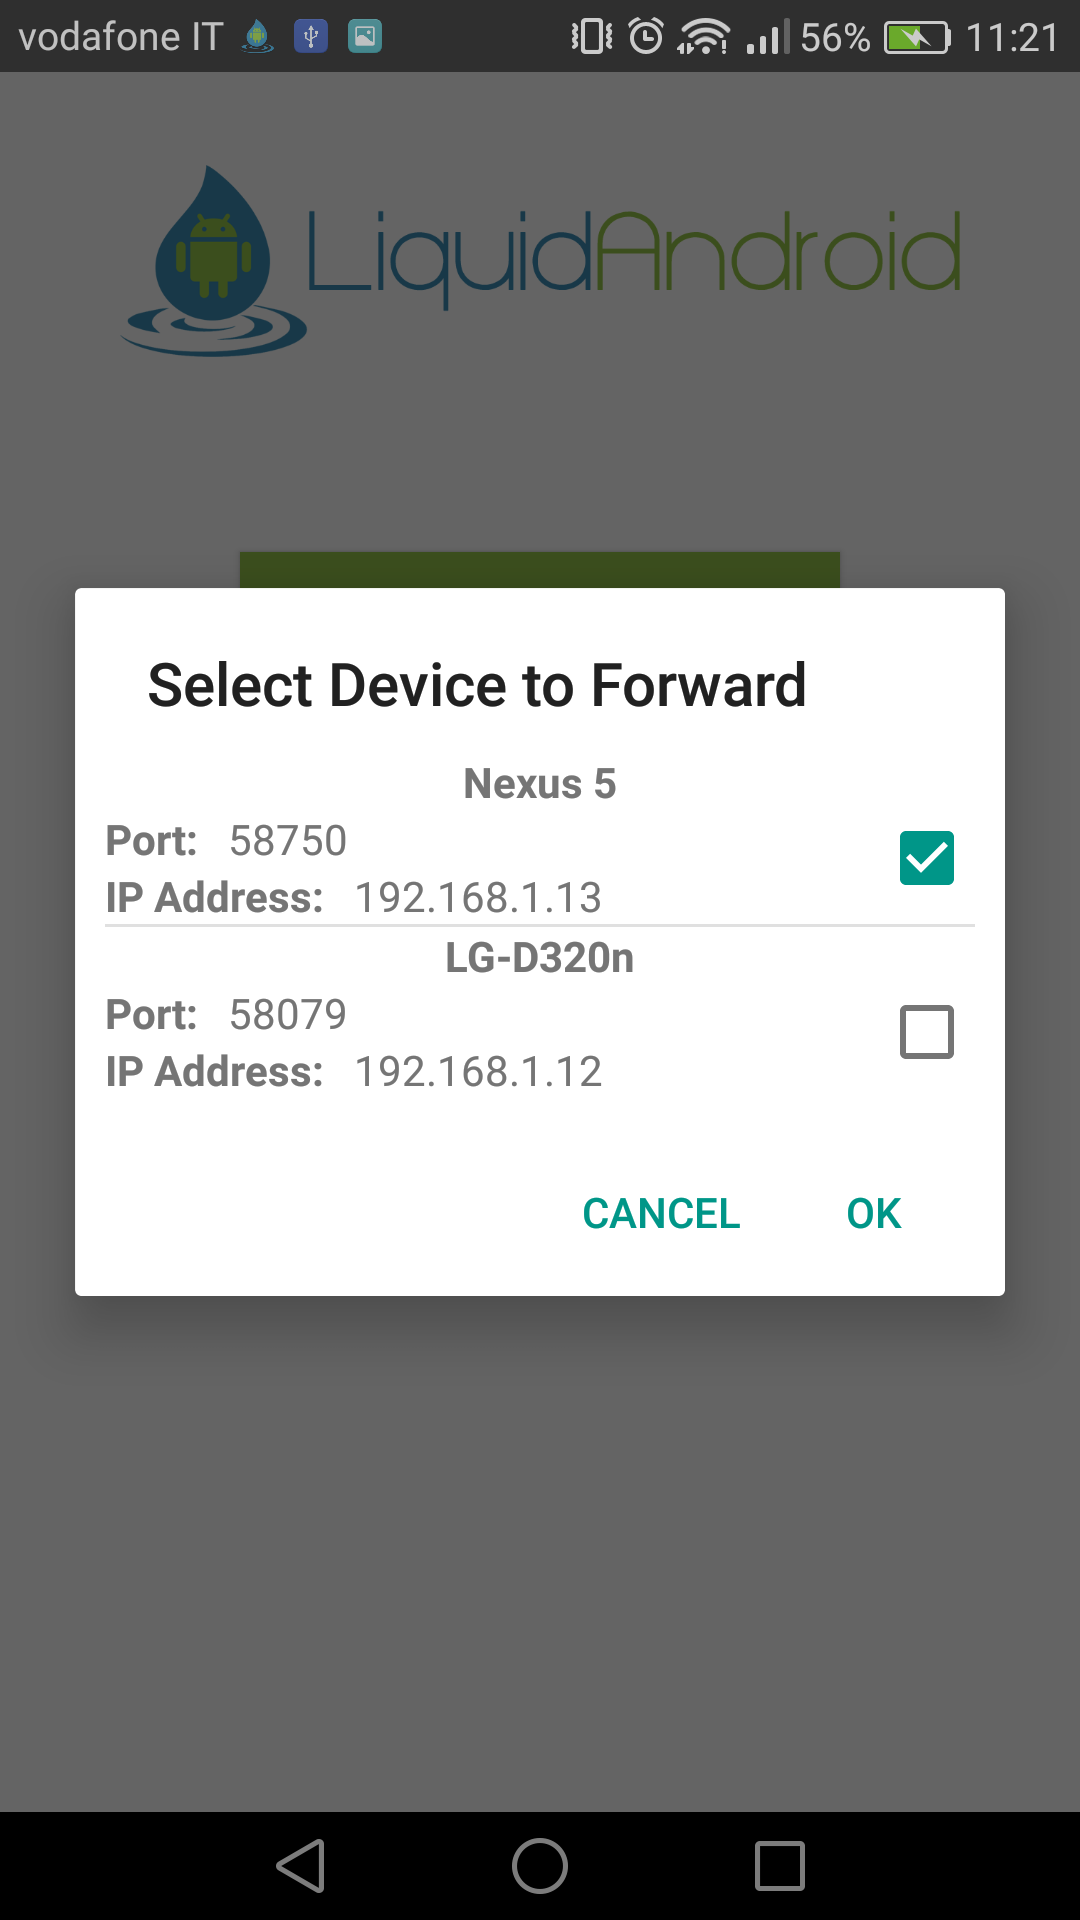
\includegraphics[width=0.75\textwidth]{alert}
		}
	\end{minipage}
	\caption{Dialogs Components}
	\label{fig:5.3}
\end{figure}
When any Android component asked the system to resolve an implicit intent, which my application can handle, the Android OS opens the \textit{App Chooser Dialog} and waits for a user choice. By selecting the Liquid Android application in the \textit{dialog} showed in \ref{subfig-1:intent}, the user ends on the MainActivity UI. Now, if the service is already in execution it can perform the forward action. The second button in the MainActivity, indeed, \textit{Forward Intent}, can be used only while the service is running. When properly clicked, it opens the \textit{Forward Dialog UI}, in \ref{subfig-2:forward}, which my middleware automatically searches for devices in the LAN with the service installed and in execution, and let the user to select on which of them forward the previously intercepted implicit intent, by ticking the \textit{check-box} as showed in the \figurename~\ref{fig:5.3}. Once selected on which device,or devices, the intent should be forwarded, by pressing the ok button, the application converts it in a JSON-Intent and sends it through the socket to them, generating Clients components which connects to the target Servers components. At this point when the message is received by the target devices, the JSON-Intent is automatically reconverted in the original Android intent, and a new intent resolution process is triggered by my application. Thus, the Android OS shows again, to the user, an \textit{App Chooser Dialog}, and lets him select with which application, among the listed ones, perform the intent task.
\begin{figure}[h]
	\centering
	\begin{minipage}{.49\textwidth}\centering
		\subfloat[App Chooser\label{subfig-1:appchooser}]{%
			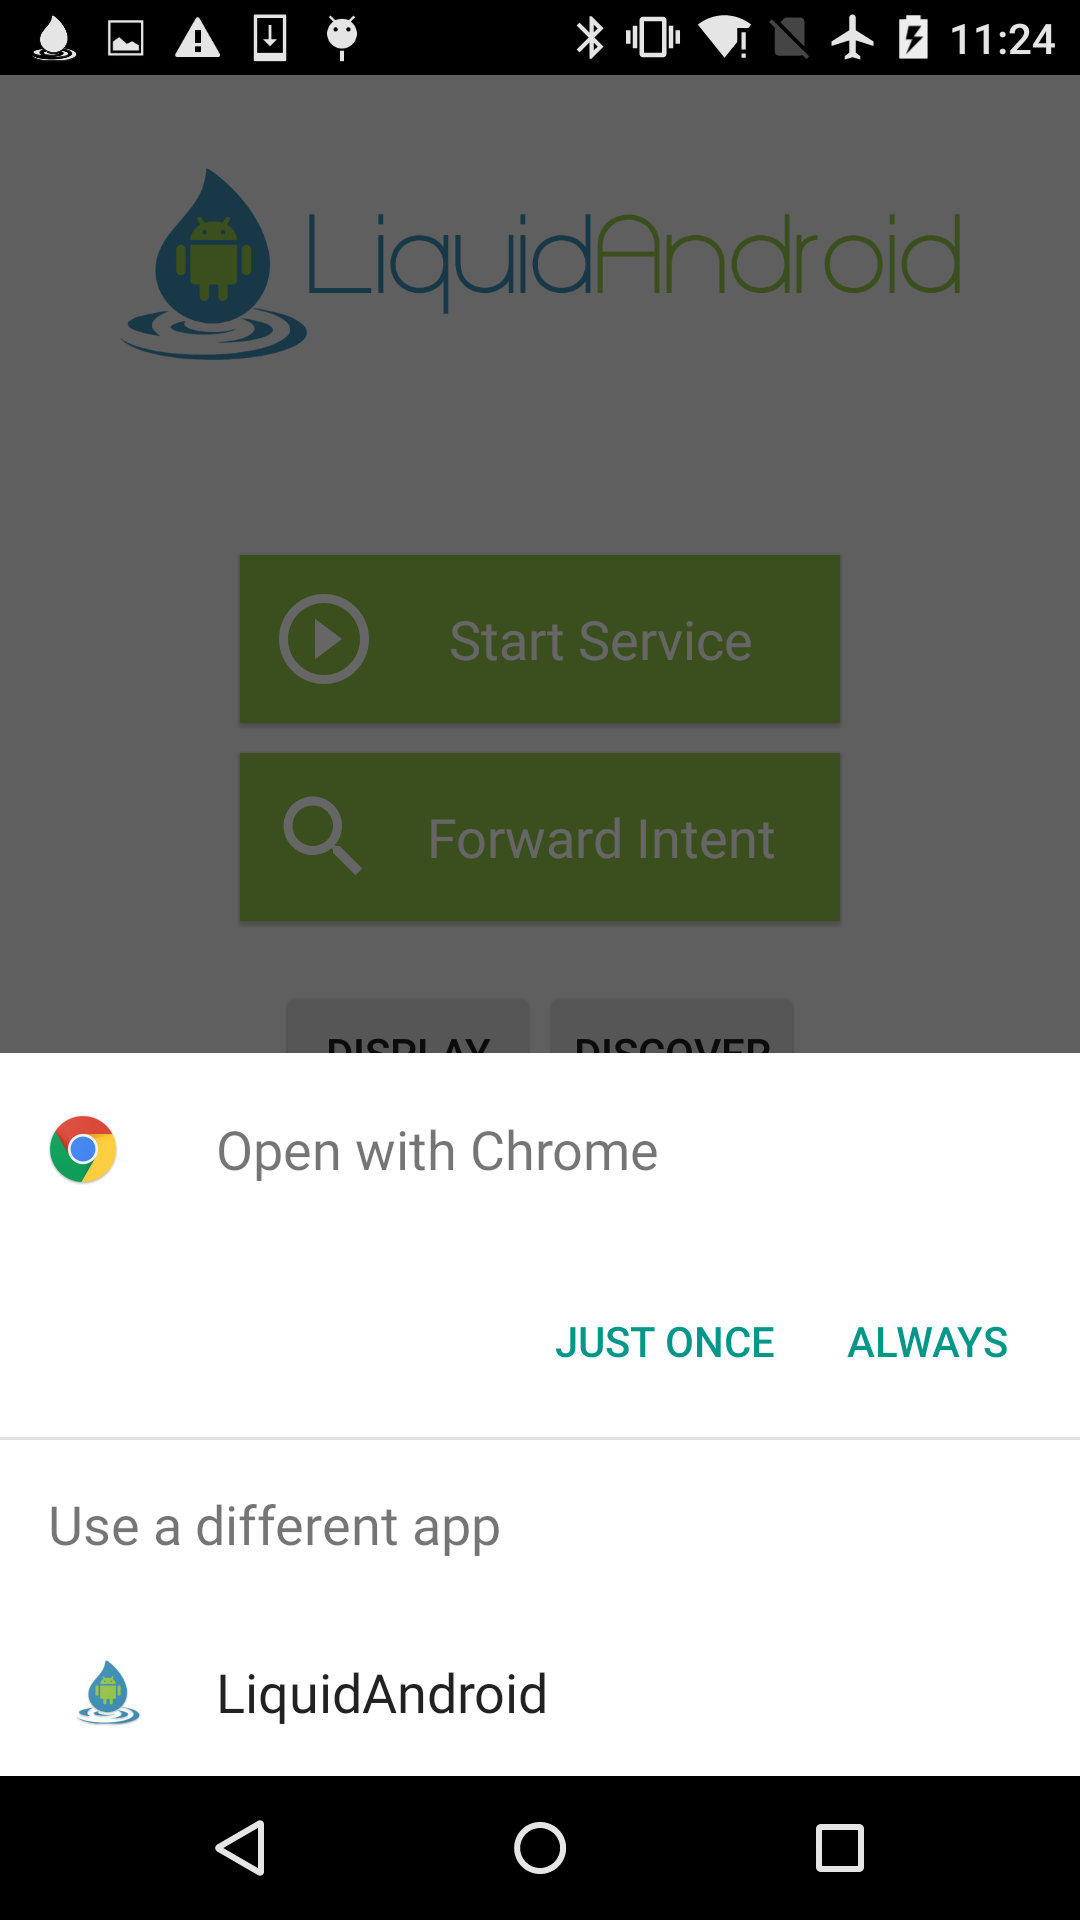
\includegraphics[width=0.75\textwidth]{appchoser}
		}
	\end{minipage}
	\begin{minipage}{.49\textwidth}\centering
		\subfloat[Third party Browser Activity\label{subfig-2:browser}]{%
			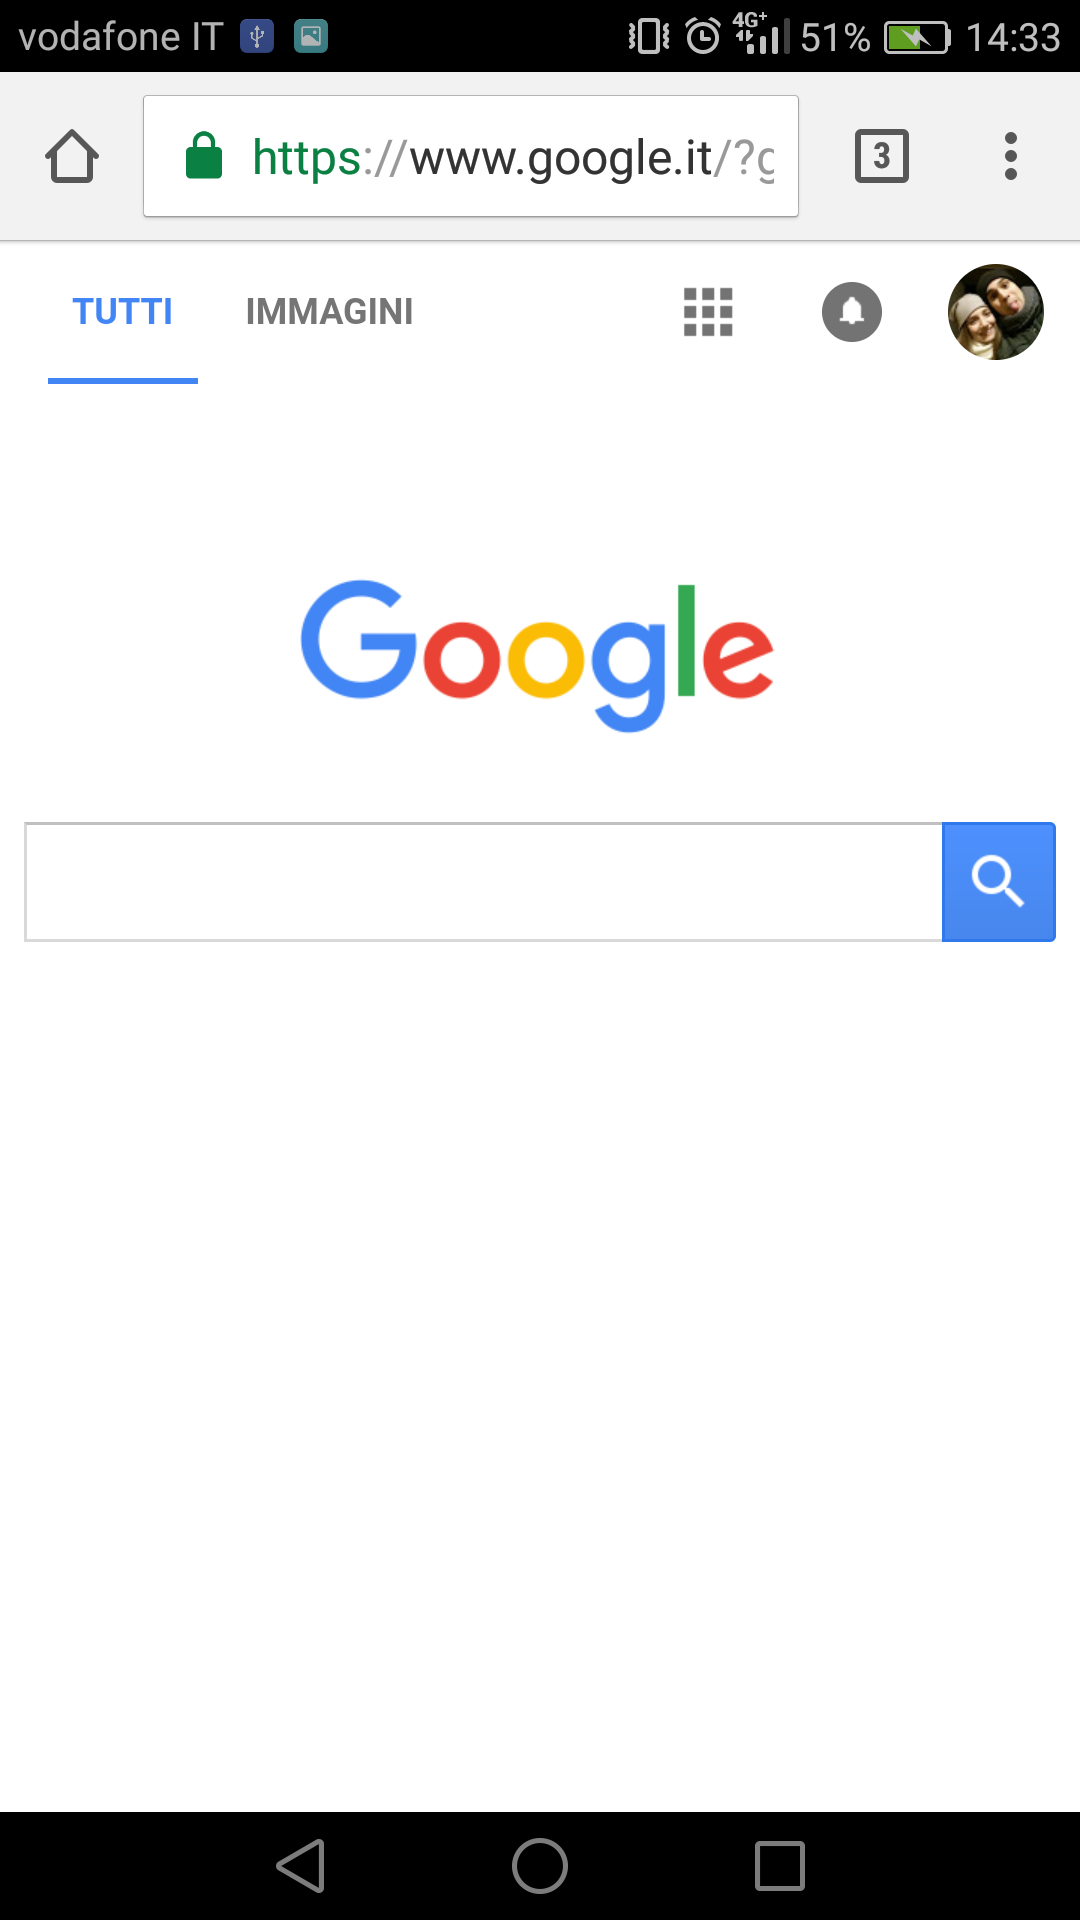
\includegraphics[width=0.75\textwidth]{browser}
		}
	\end{minipage}
	\caption{JSON-Intent execution}
	\label{fig:5.4}
\end{figure}
The \figurename~\ref{fig:5.4} describes the working mechanism above explained, in this particular case the devices received an intent to view the web-page \textit{http://Google.it}. By selecting, in \ref{subfig-1:appchooser}, \textit{Open with Chrome}, the process terminates with the execution of the browser activity, in \ref{subfig-2:browser}, showing exactly that page.

\subsection{Live Test Cases}
In this subsection I want to present two live tests I performed to prove that my application respects all the constrains and fulfill all the functional, and also non-functional, requirements.
As already explained, I created a second simple Android application working as a client for the Liquid Android middleware. This application \textit{Intent Generator} is composed by a single activity in which there are some buttons to let the user create easily implicit intents to be resolved by the Android OS.
\begin{figure}[h]
	\centering
	\begin{minipage}{.49\textwidth}\centering
		\subfloat[Intent Generator MainActivity\label{subfig-1:intentmain}]{%
			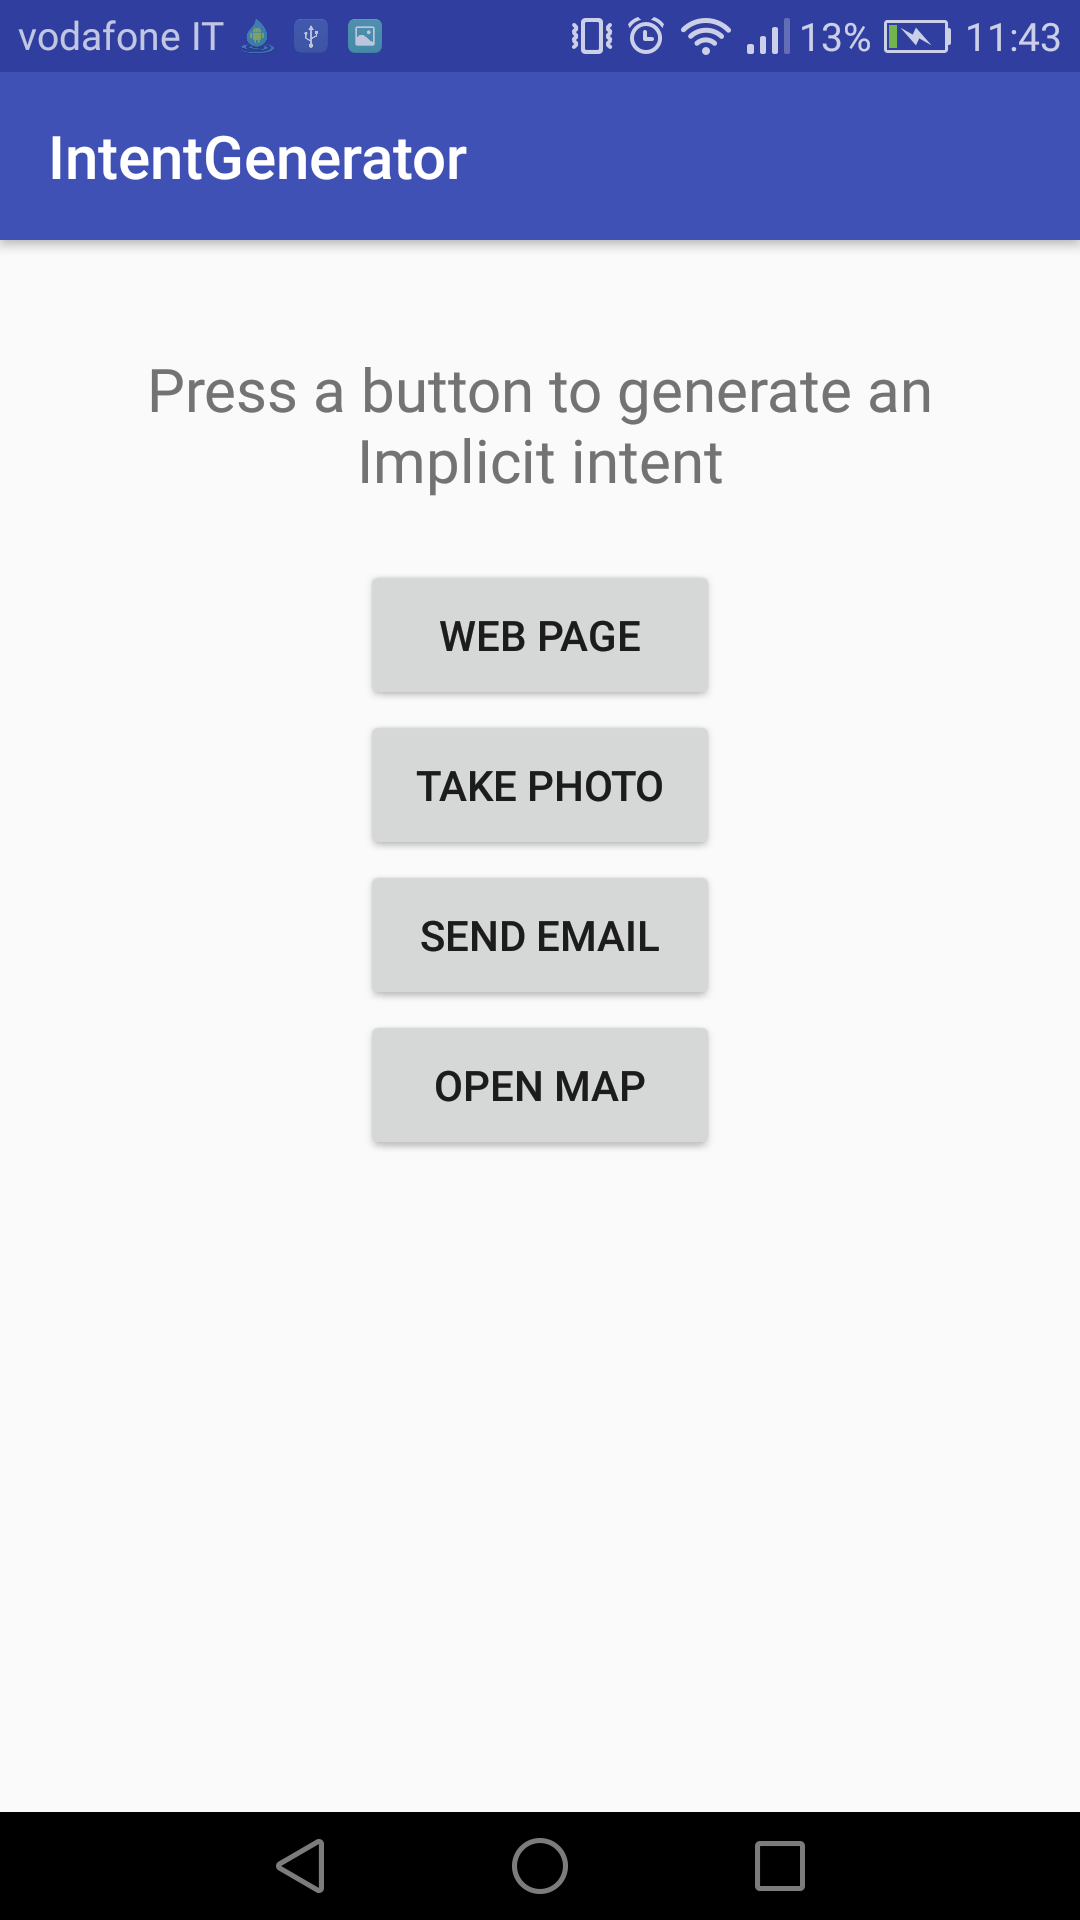
\includegraphics[width=0.75\textwidth]{intentgenerator}
		}
	\end{minipage}
	\begin{minipage}{.49\textwidth}\centering
		\subfloat[Intent Generator data Picker\label{subfig-2:picker}]{%
			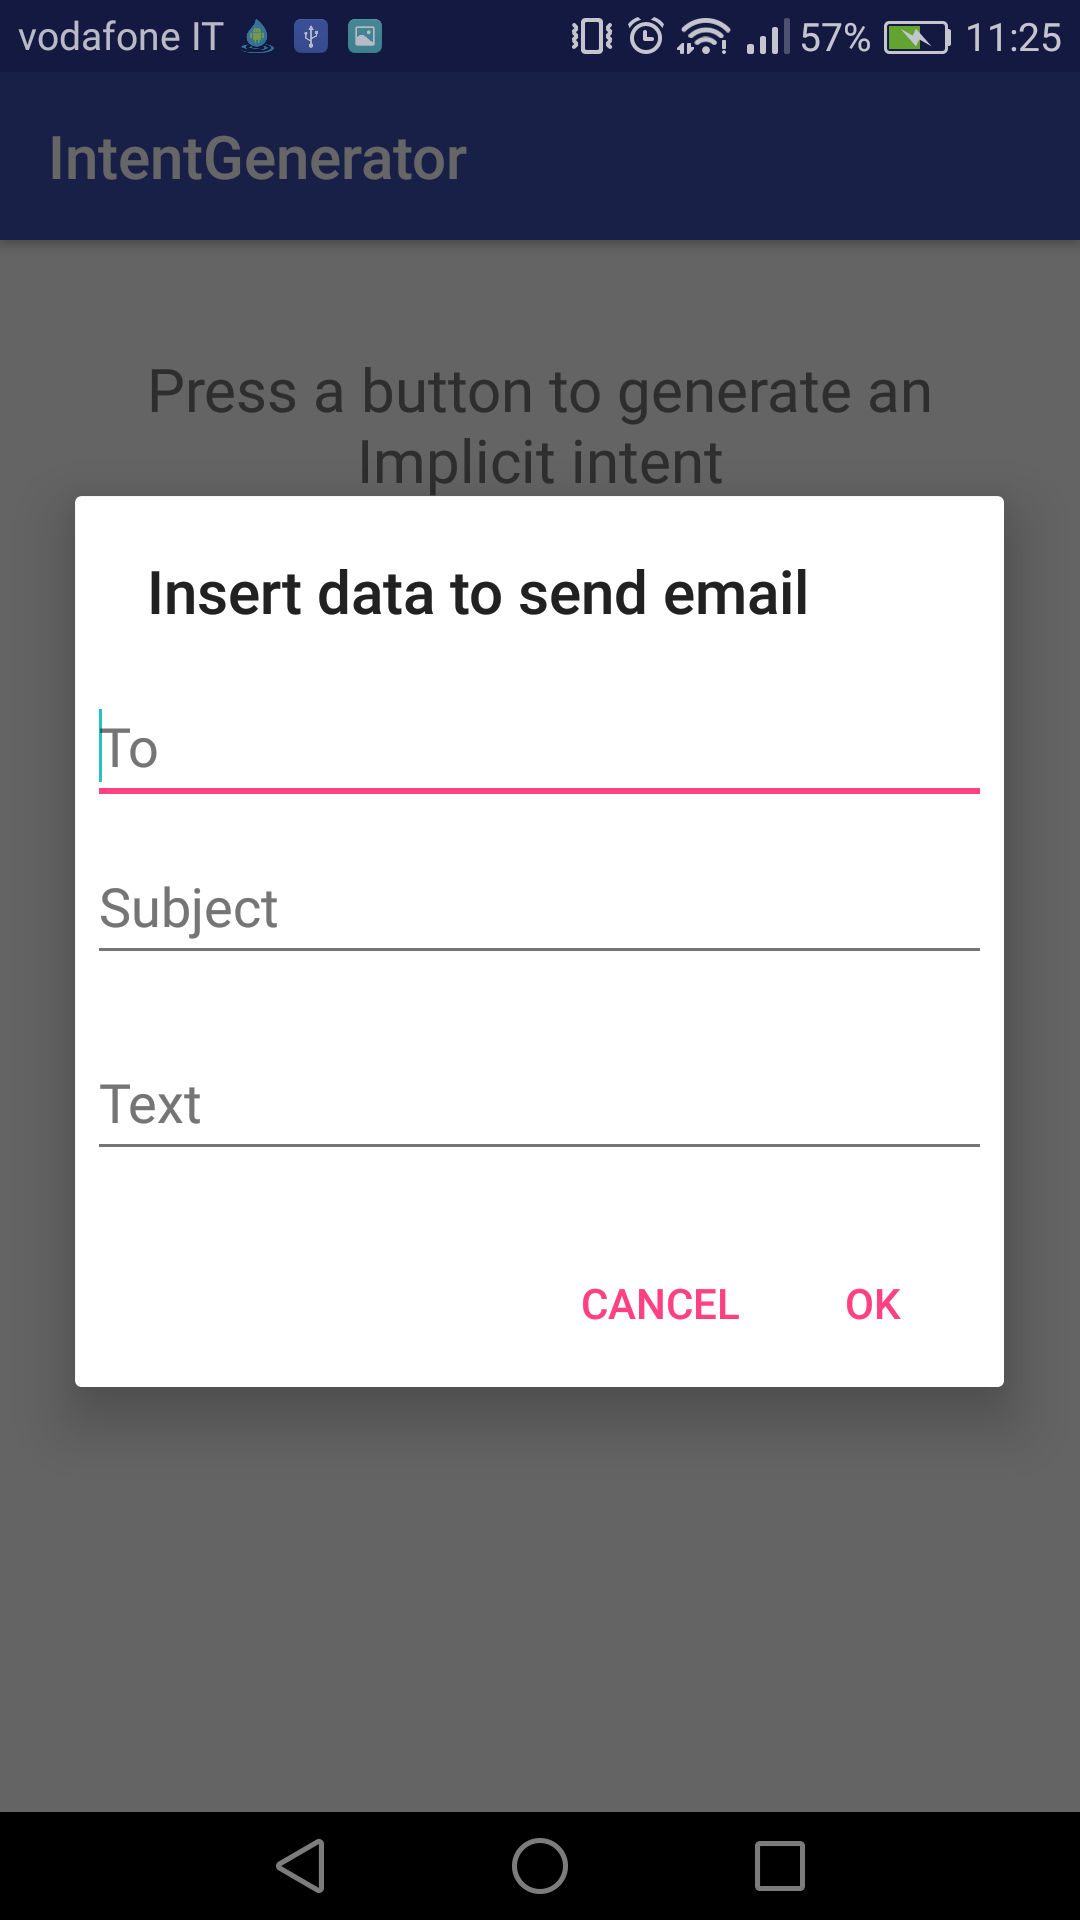
\includegraphics[width=0.75\textwidth]{picker}
		}
	\end{minipage}
	\caption{Intent Generator UI}
	\label{fig:5.5}
\end{figure}
In \figurename~\ref{fig:5.5} there are two screenshots of the \textit{Intent Generator} application. In \ref{subfig-1:intentmain}, there is the main activity, with which I generate some common implicit intents, to be forwarded using the Liquid Android middleware, by simply pressing the desired button in the UI. When the intent to be generated needs extra data the applications shows a \textit{Dialog Picker} to let insert additional data to the intent, as shown, in \ref{subfig-2:picker}, when the \textit{SEND EMAIL} button is pressed.\\
By using this environment I have performed the tests I am presenting in this section. Both test cover all the functionalities the systems must have, taking in to account, also the data management problem. The first test is use the system to forward an intent to send a text email from one device to another in the system. The second one is a bit more complicated, one device of the network ask two other devices to take a picture with their camera and then to have the taken photos back.
\subsubsection{Send Email Live Test}
In this live test scenario I assume that there are two Android devices, with the Liquid Android middleware application already installed and with the service in execution.
In \figurename~\ref{fig:5.6} it is shown the complete UML sequence diagram, which completely describes this live test.\\
The first device starts the process by using the Intent Generator MainActivity, precisely by pressing the \textit{SEND EMAIL} button, already shown in \ref{subfig-1:intentmain}. Then he compiles the fields in the dialog and, once done, the implicit intent is created by the application and passed to the Android OS. The OS looks for activities capable of handling the so generated intent, and ask the user, by showing the App Chooser, with which compatible application he wants to resolve the intent. In this case the user selects the liquid android application, and ends on its MainActivity.\\
At this point the \textit{Forward Intent button} is pressed and the intent is automatically converted and sent to the selected device/s. When the intent arrives to the target, the Liquid Android Service reconverts it in an intent object to be executed and passes it to the OS.
\begin{figure}[h]
	\centering
	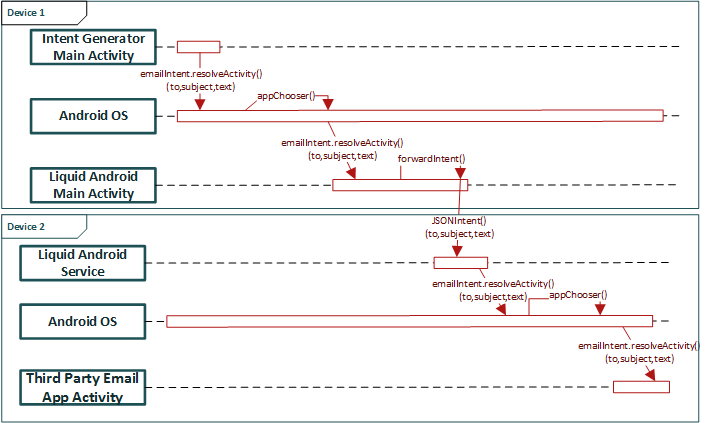
\includegraphics[width=1\textwidth]{sequence1}
	\caption{Live test 1 Sequence Diagram}
	\label{fig:5.6}
\end{figure}
The Android OS starts again a resolution process and at the end shows again the App Chooser. Now the user selects the Gmail application and completes the action by sending the email from the Gmail activity, already filled with the data the user inserted in the first device.\\
In \figurename~\ref{fig:5.7} there is the complete flow of actions presented with some real screenshots of the applications I have developed. In particular the screens from \textit{a} to \textit{d} are taken from the first device I have used, a Huawei P9, and screens \textit{e} and \textit{f} are taken from the target device, a LG L70.
\\\\
\begin{figure}[h]
	\centering
	\begin{minipage}{.24\textwidth}\centering
		\subfloat[Send Email\label{subfig-1:intentg}]{%
			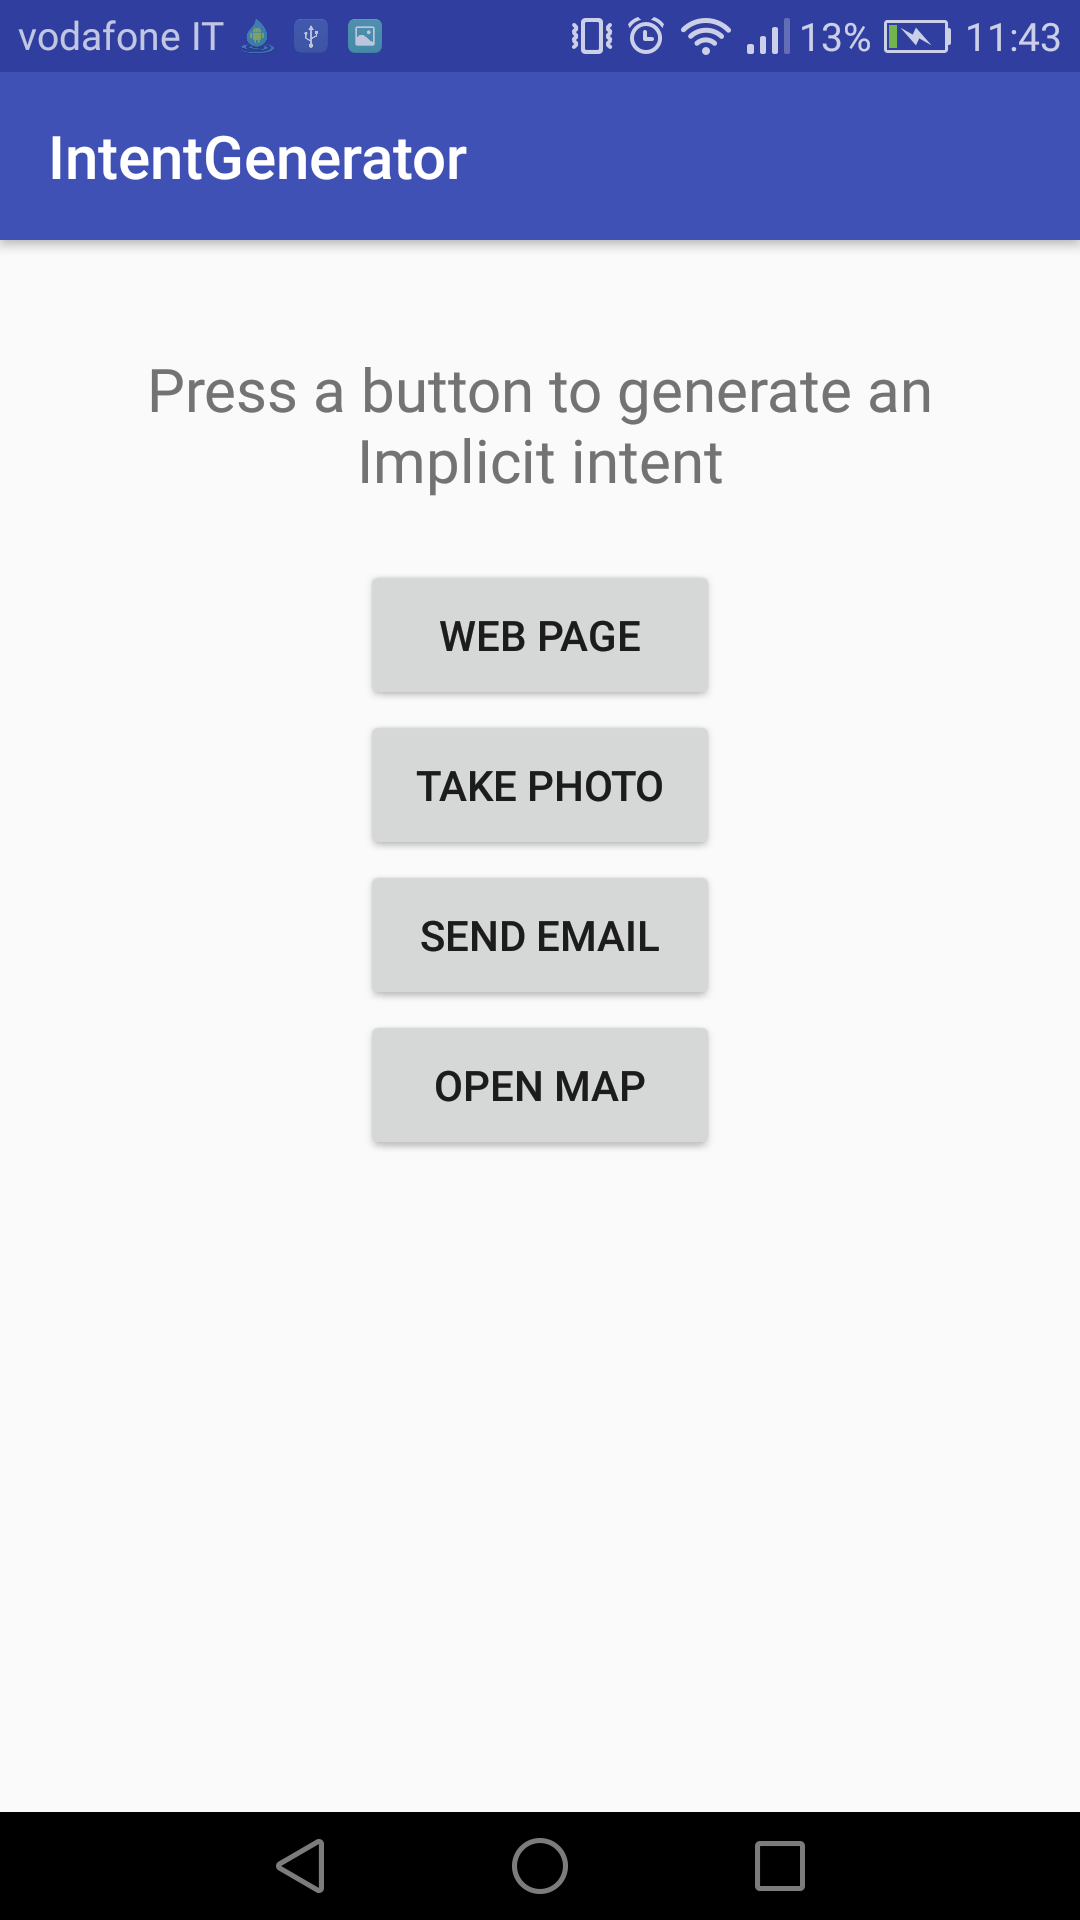
\includegraphics[width=0.9\textwidth]{intentgenerator}
		}
	\end{minipage}
	\begin{minipage}{.24\textwidth}\centering
		\subfloat[Picker Dialog\label{subfig-2:chooser}]{%
			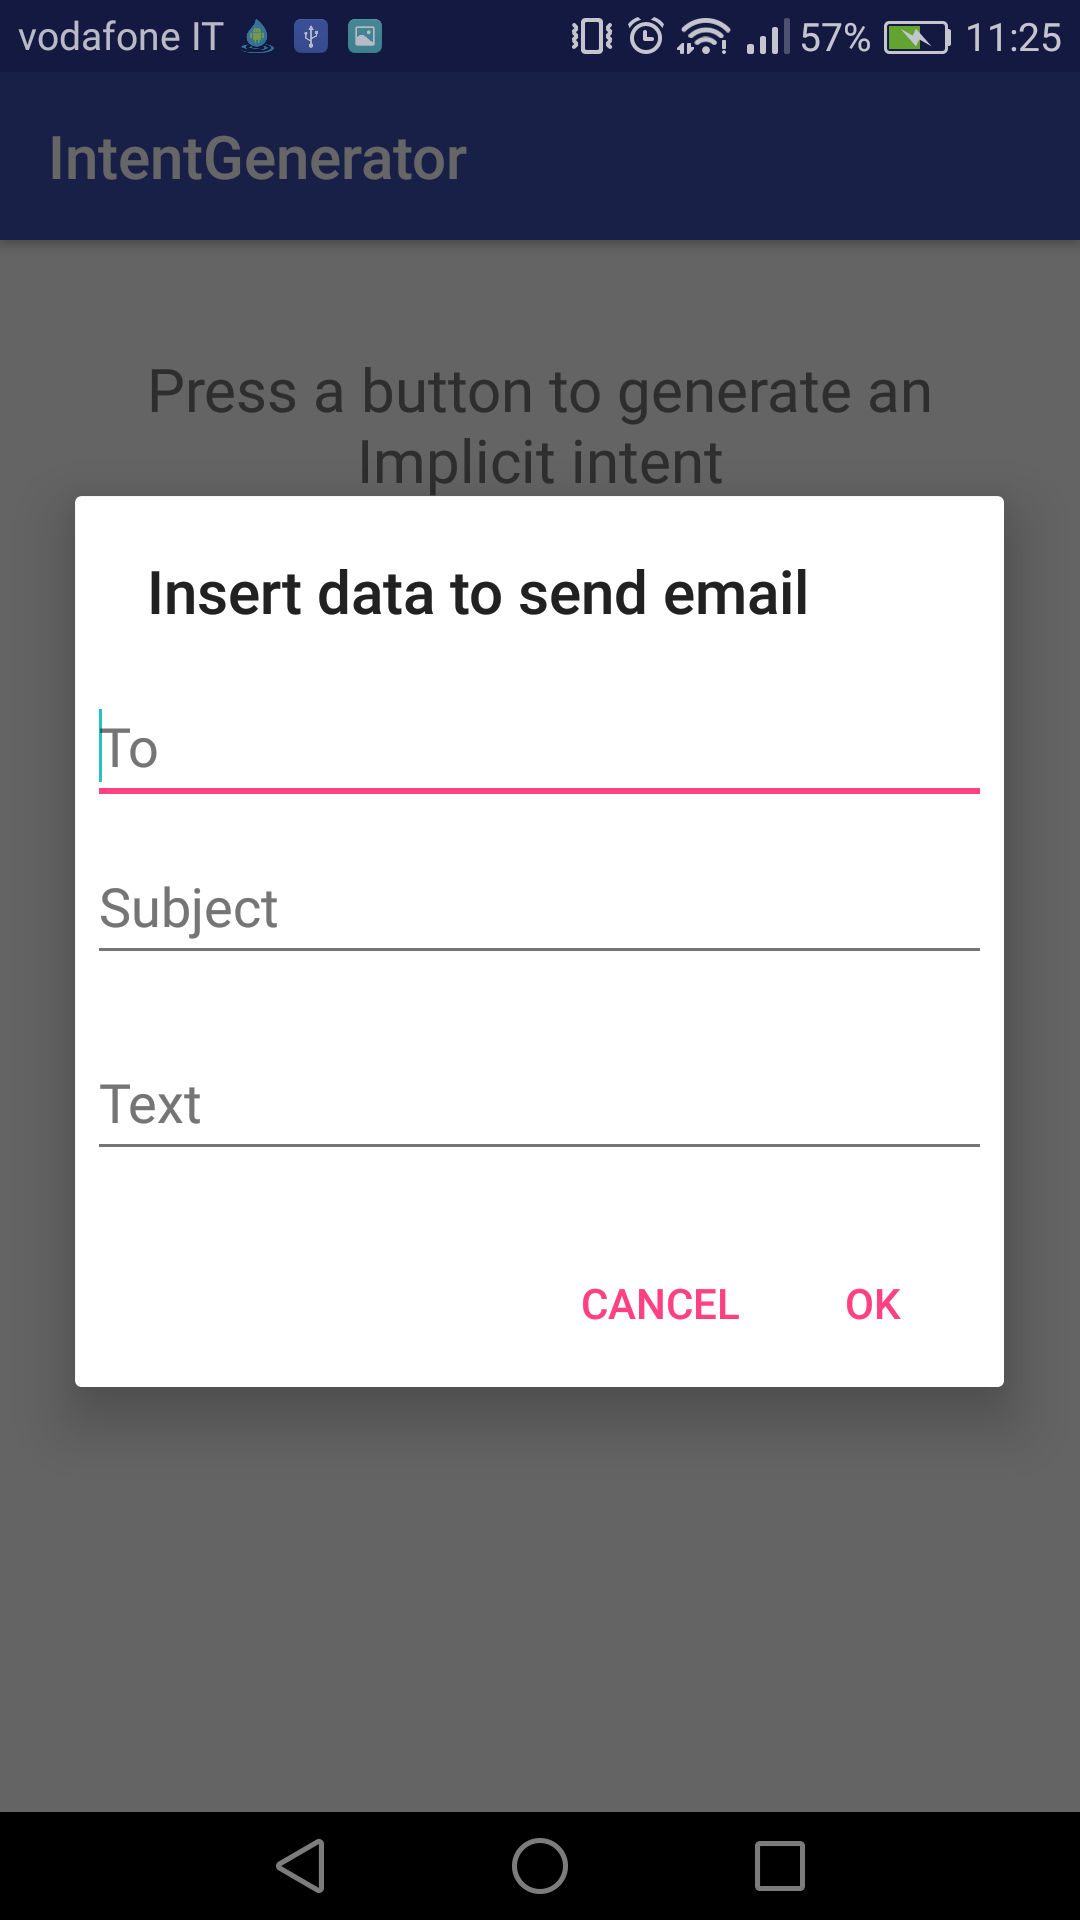
\includegraphics[width=0.9\textwidth]{picker}
		}
	\end{minipage}
	\centering
	\begin{minipage}{.24\textwidth}\centering
		\subfloat[App Chooser\label{subfig-3:liquid}]{%
			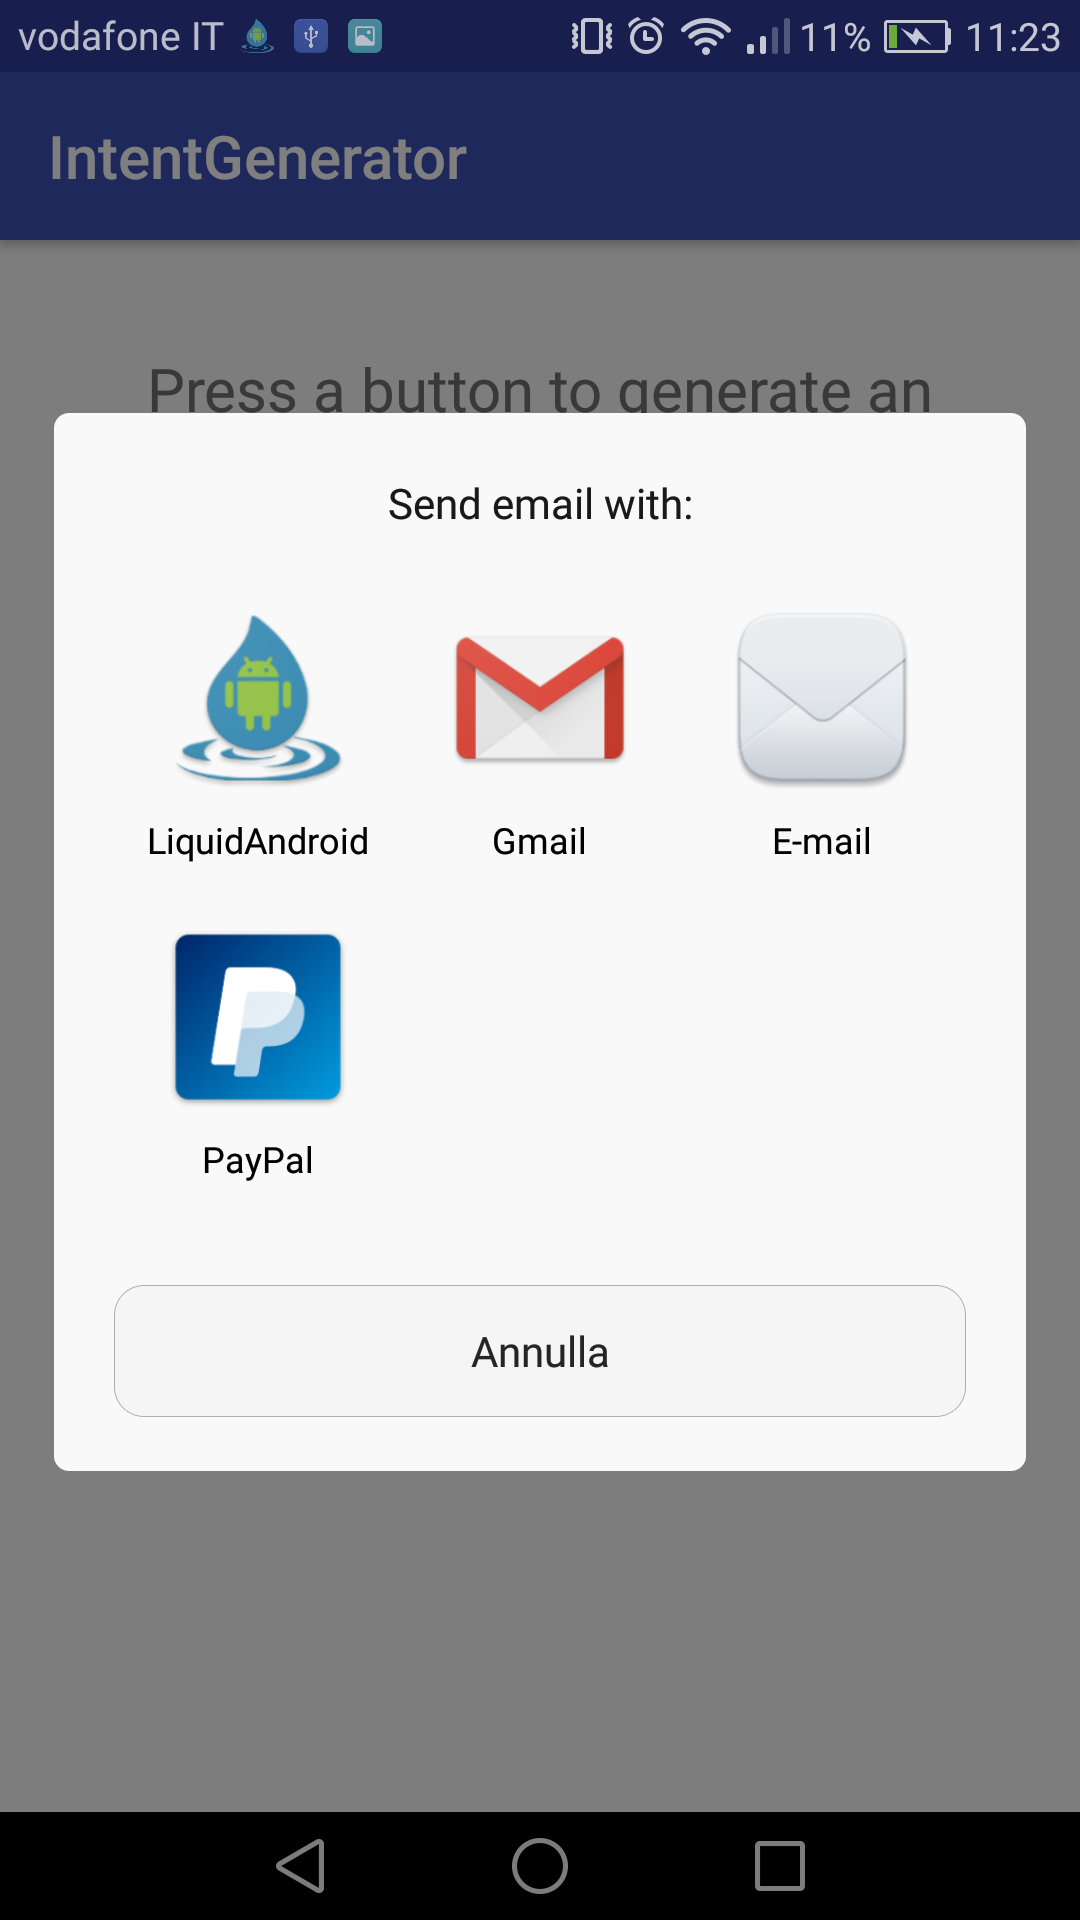
\includegraphics[width=0.9\textwidth]{sendwith}
		}
	\end{minipage}
	\begin{minipage}{.24\textwidth}\centering
		\subfloat[Forward Dialog\label{subfig-4:chooser2}]{%
			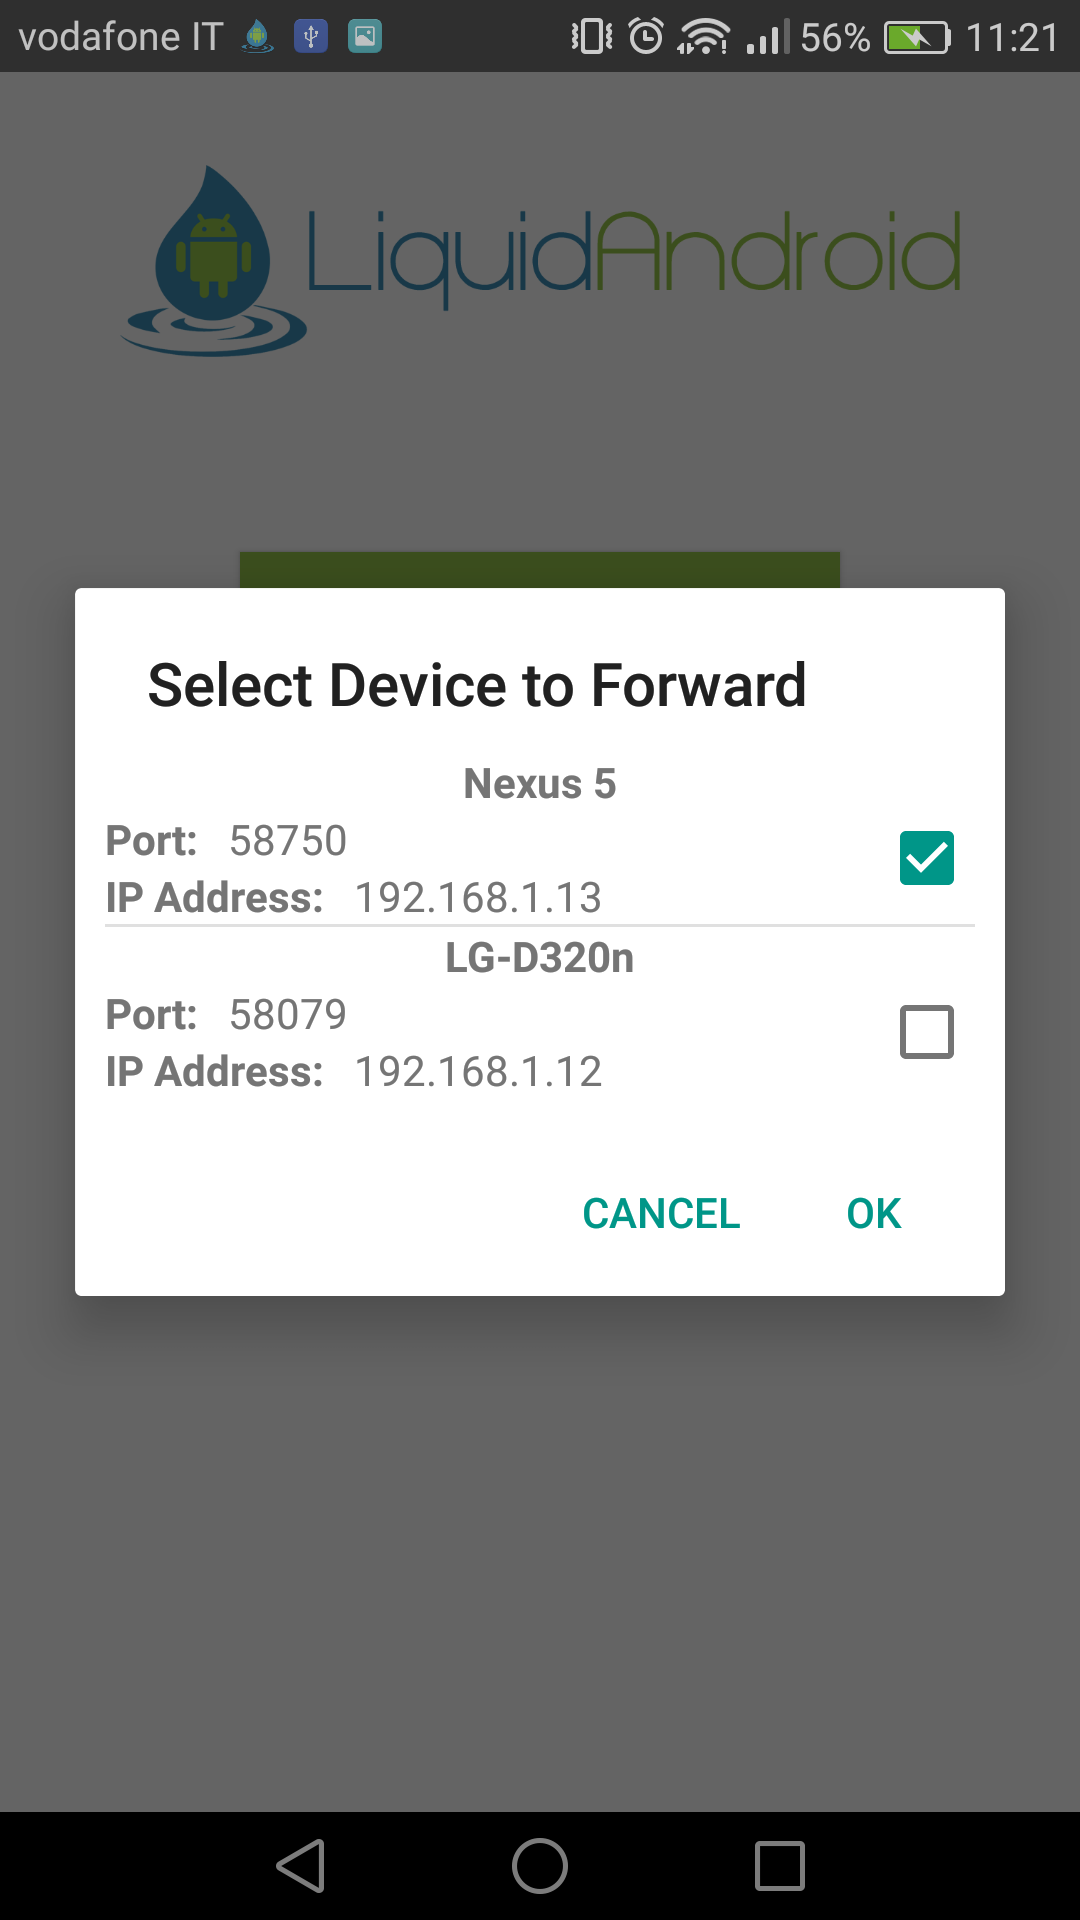
\includegraphics[width=0.9\textwidth]{alert}
		}
	\end{minipage}
	\phantomcaption 
	\label{fig:5.7}
\end{figure}

\begin{figure}[h]
\ContinuedFloat
\centering
\begin{minipage}{.24\textwidth}\centering
	\bigskip
	\subfloat[App Chooser\label{subfig-5:chooser2}]{%
		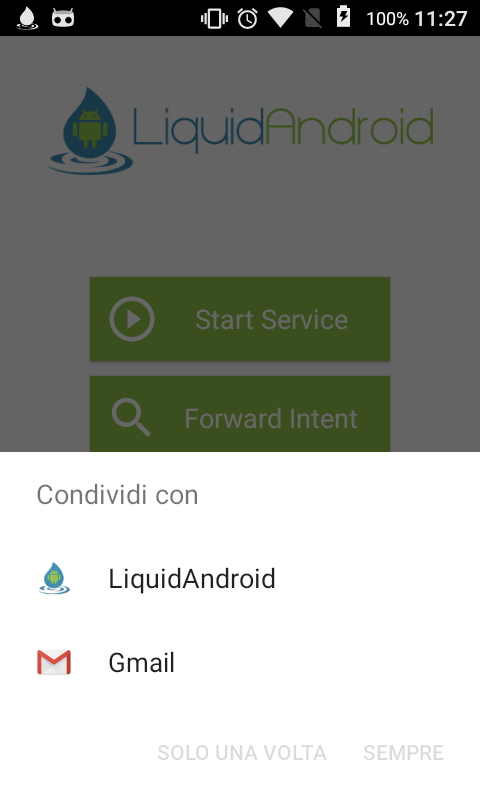
\includegraphics[width=0.9\textwidth]{condividicon}
	}
\end{minipage}
\begin{minipage}{.24\textwidth}\centering
	\bigskip
	\subfloat[Gmail Activity\label{subfig-6:chooser}]{%
		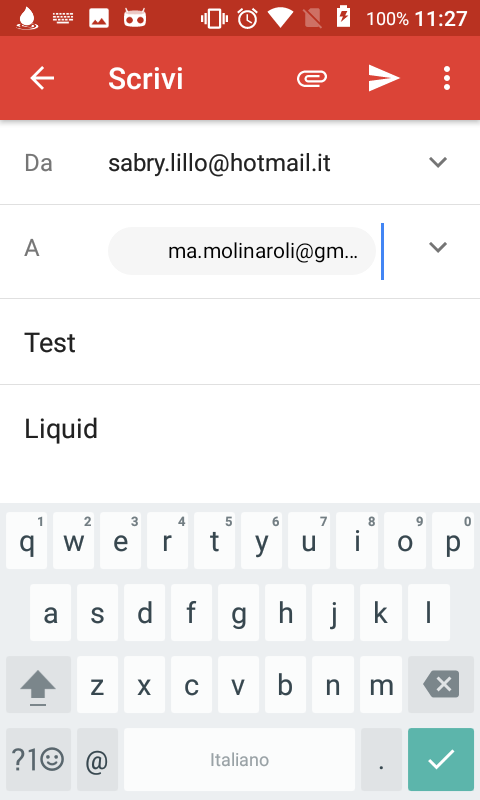
\includegraphics[width=0.9\textwidth]{gmail}
	}
\end{minipage}
\caption{Complete email live test screenshots}
\end{figure}
\subsubsection{Take Photo Live Test}
The second test I want to report exploits the Android \textit{startActivityforResult()} mechanism: it handles more complex data, and returns them to the caller. The environment I have used is exactly the one described in the previous test: three Android devices connected in the same LAN with the Liquid Android application already installed, and the background service already in execution. I want to prove that the middleware can work with more than two devices and how it manages concurrent requests. To do this I want that one device in the network, ask the other two devices to pick a photo at the same time, and once done, send the two different picture, taken with two different devices, to the original caller. I started the test by using the Intent Generator app, to generate the photo intent. When the intent is triggered the Android OS opens the app Chooser, showing the Liquid Android application as an alternative to resolve the intent. I have forwarded the intent, using the forward button, and sent it to the other two devices in the network. Once the intent arrived, the Liquid Android service triggers it, and passes it to the Liquid Android Result Activity, which starts the Android camera waiting for results. Once the user have taken the photo, with the camera, the Results Activity brings it, and send the picture back to the caller. When the picture arrives back to the caller the Liquid Android application, shows it in its Result activity. Since the intent was forwarded in two devices, when the two picture are sent back to the caller, the two result are concurrent. My system allows that concurrency by accepting different calls using different threads and then it puts in foreground the last call arrived using a LIFO policy. This complete test scenario is described, as done with the other test, showing the interaction of the components, and their activation in the UML sequence diagram in \figurename~\ref{fig:5.8}. In the diagram only two devices are present, but the third device involved in the test has exactly the same behavior the \textit{device 2} showed in the picture.\\\\\\\\
\begin{figure}[h]
	\centering
	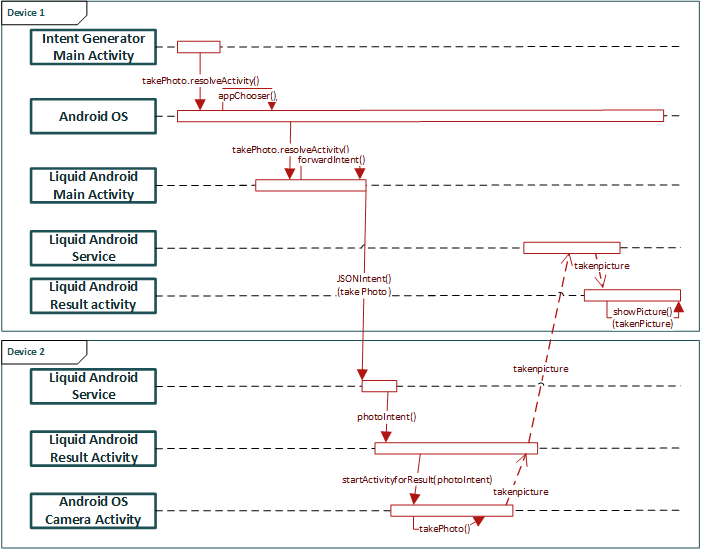
\includegraphics[width=1\textwidth]{sequence2}
	\caption{Live test 2 Sequence Diagram}
	\label{fig:5.8}
\end{figure}\\
As already done with the previous live test case, I want to provide a set of screenshots showing the application behavior while running this example.\\
In \figurename~\ref{fig:5.9} there is the complete flow of actions presented with some real screenshots of the applications I have developed. In particular the screens from \textit{a} to \textit{c} are taken from the first device I have used, a Huawei P9, to generate and forward the so called photo intent.\\
\begin{figure}[h!]
	\centering
	\begin{minipage}{.24\textwidth}\centering
		\subfloat[Send Email\label{subfig-1:intentg2}]{%
			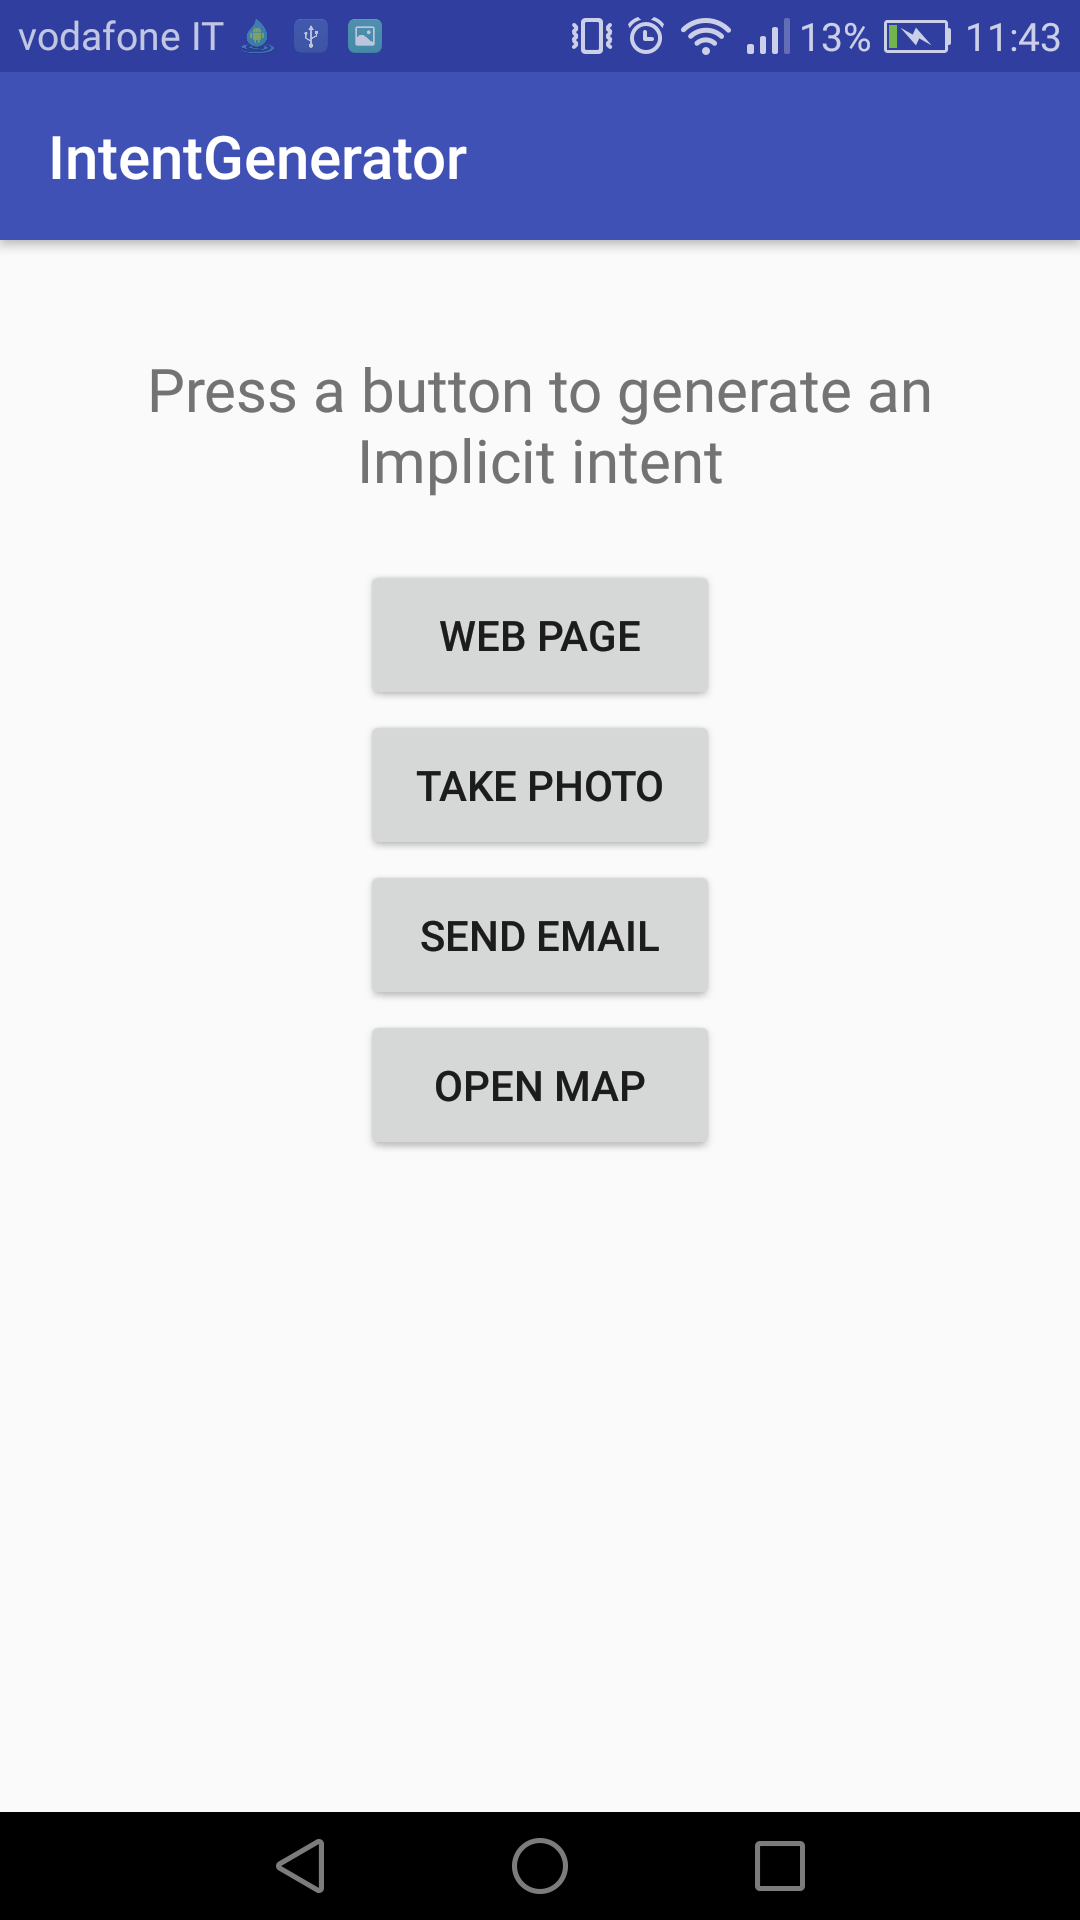
\includegraphics[width=0.9\textwidth]{intentgenerator}
		}
	\end{minipage}
	\begin{minipage}{.24\textwidth}\centering
		\subfloat[App Chooser\label{subfig-2:chooser2}]{%
			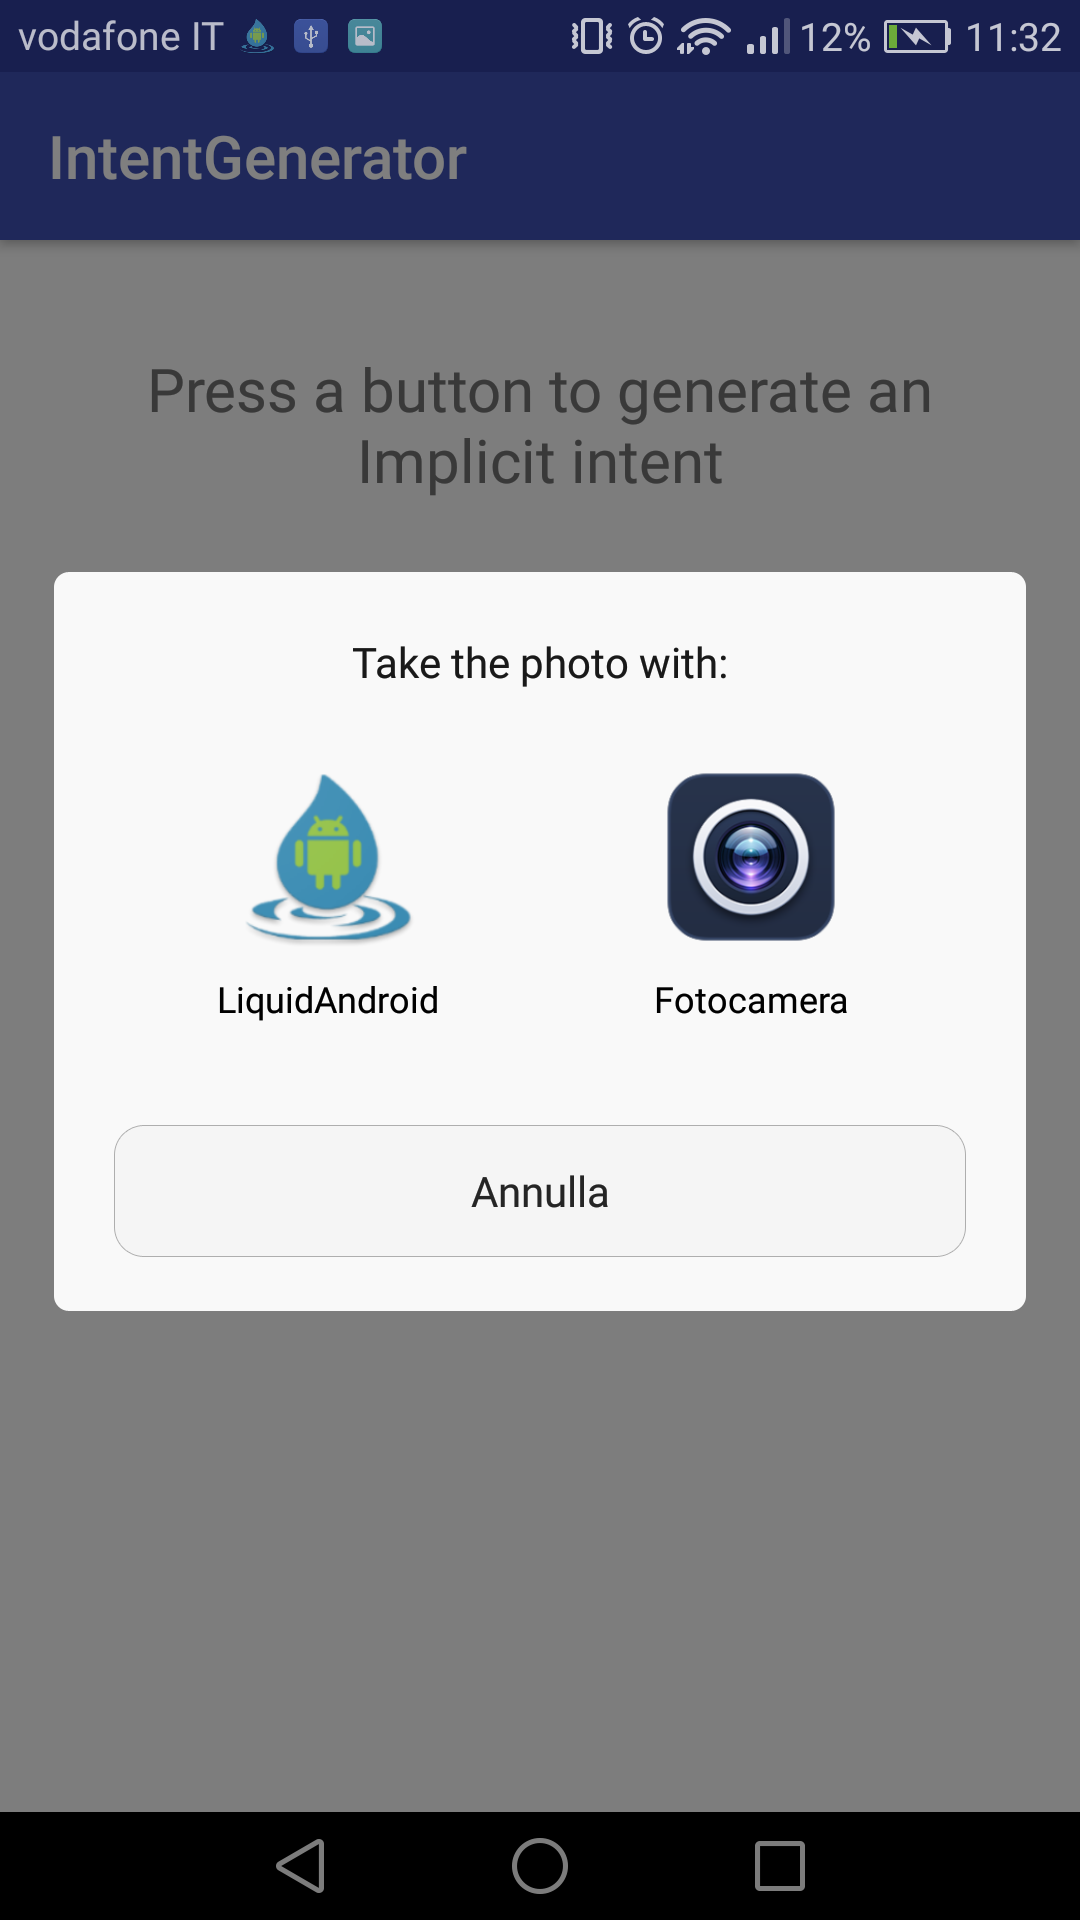
\includegraphics[width=0.9\textwidth]{photochooser}
		}
	\end{minipage}
	\centering
	\begin{minipage}{.24\textwidth}\centering
		\subfloat[Forward Dialog\label{subfig-3:liquid2}]{%
			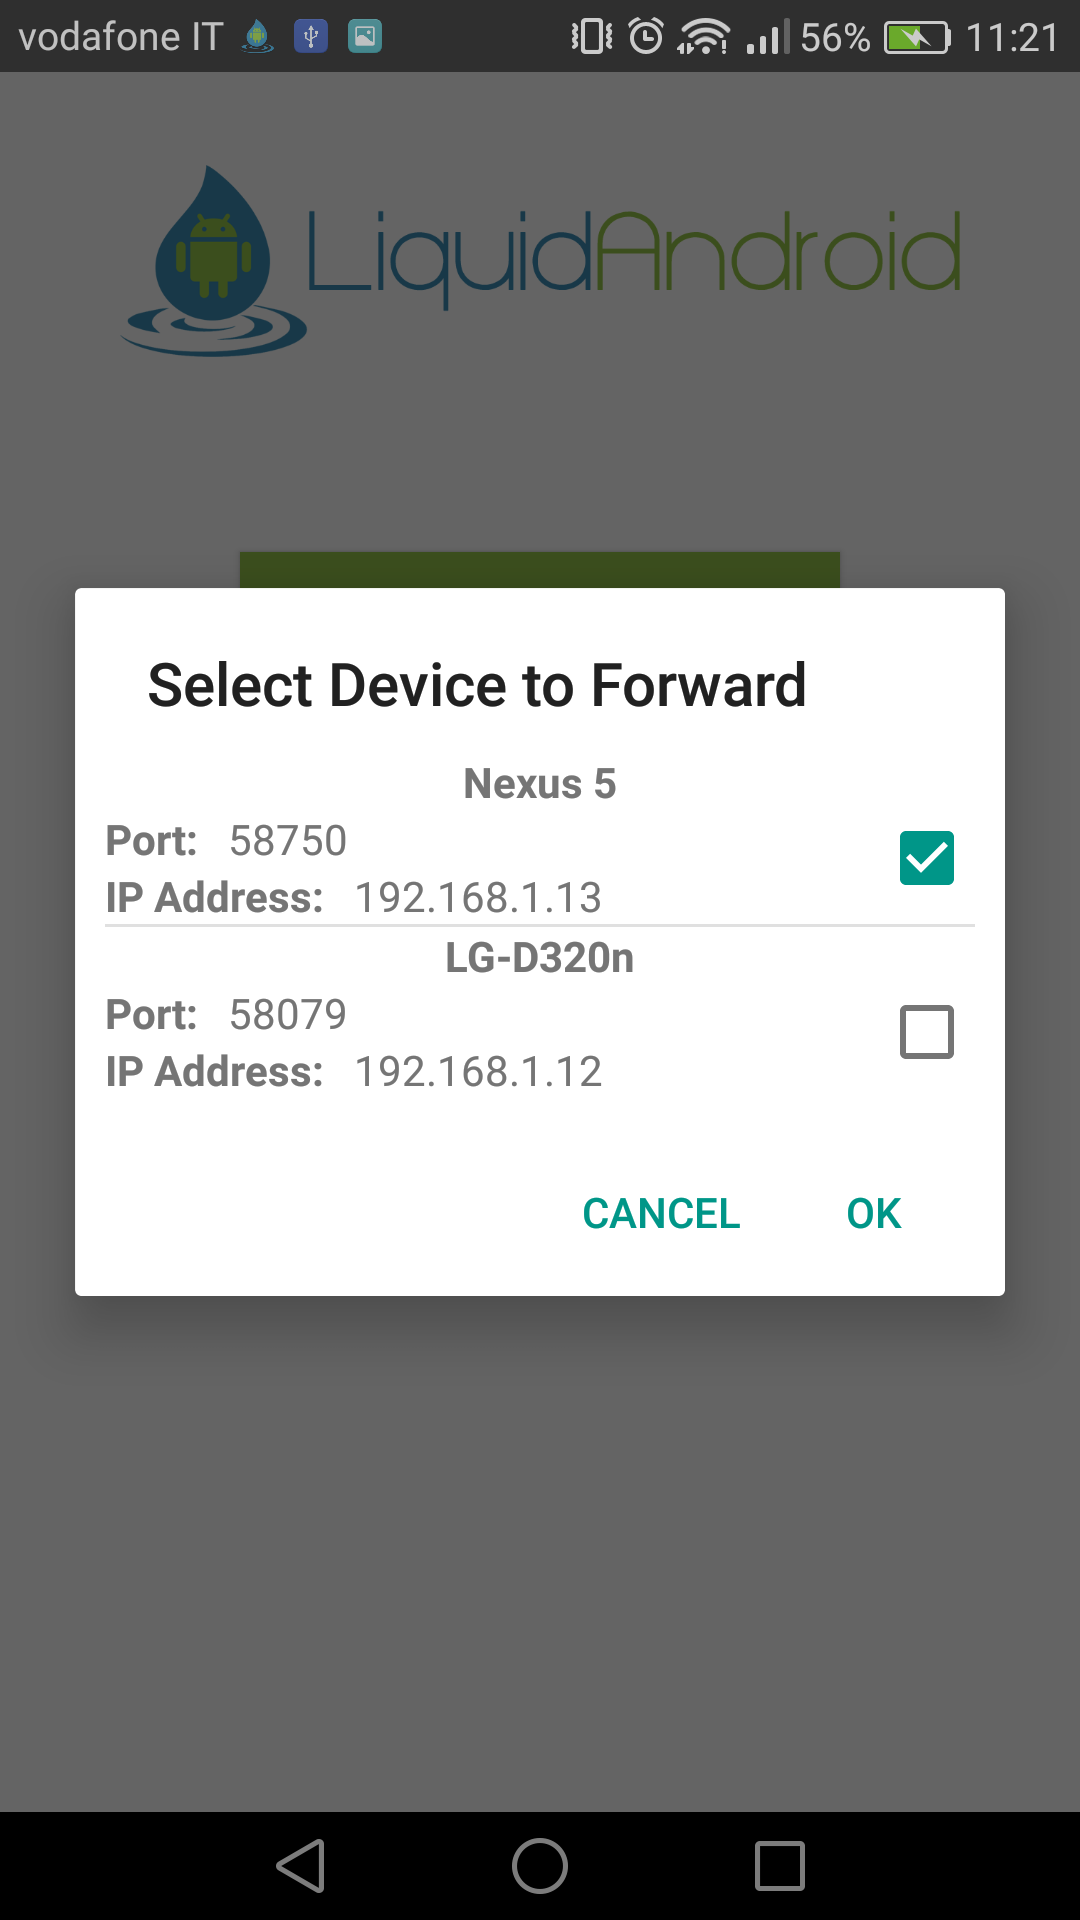
\includegraphics[width=0.9\textwidth]{alert}
		}
	\end{minipage}
	\begin{minipage}{.24\textwidth}\centering
		\subfloat[App Chooser\label{subfig-4:chooser3}]{%
			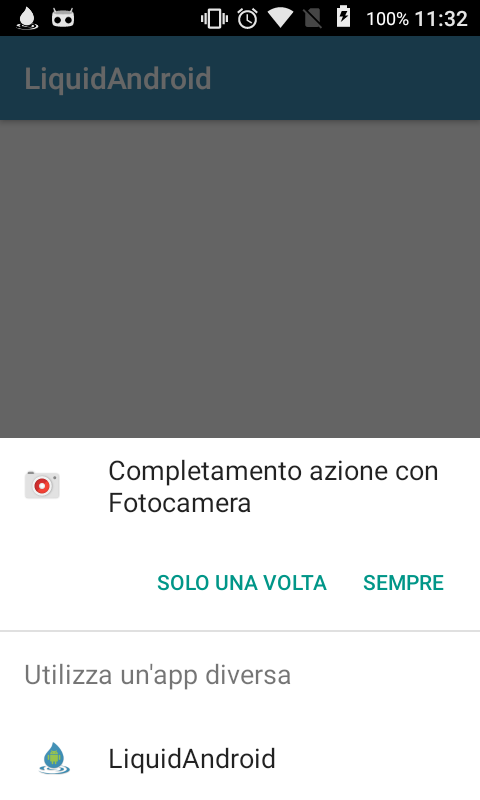
\includegraphics[width=0.9\textwidth]{chosphoto2}
		}
	\end{minipage}
	\phantomcaption
	\label{fig:5.9}
\end{figure}
\begin{figure}[h!]
	\ContinuedFloat
	\centering
	\begin{minipage}{.24\textwidth}\centering
		\bigskip
		\subfloat[Android Camera\label{subfig-5:camera2}]{%
			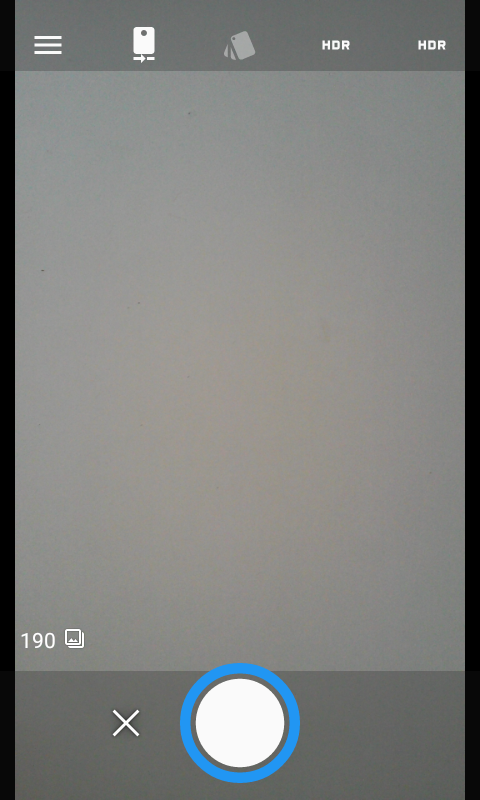
\includegraphics[width=0.9\textwidth]{camera2}
		}
	\end{minipage}
	\begin{minipage}{.24\textwidth}\centering
		\bigskip
		\subfloat[App Chooser\label{subfig-6:chooser2}]{%
			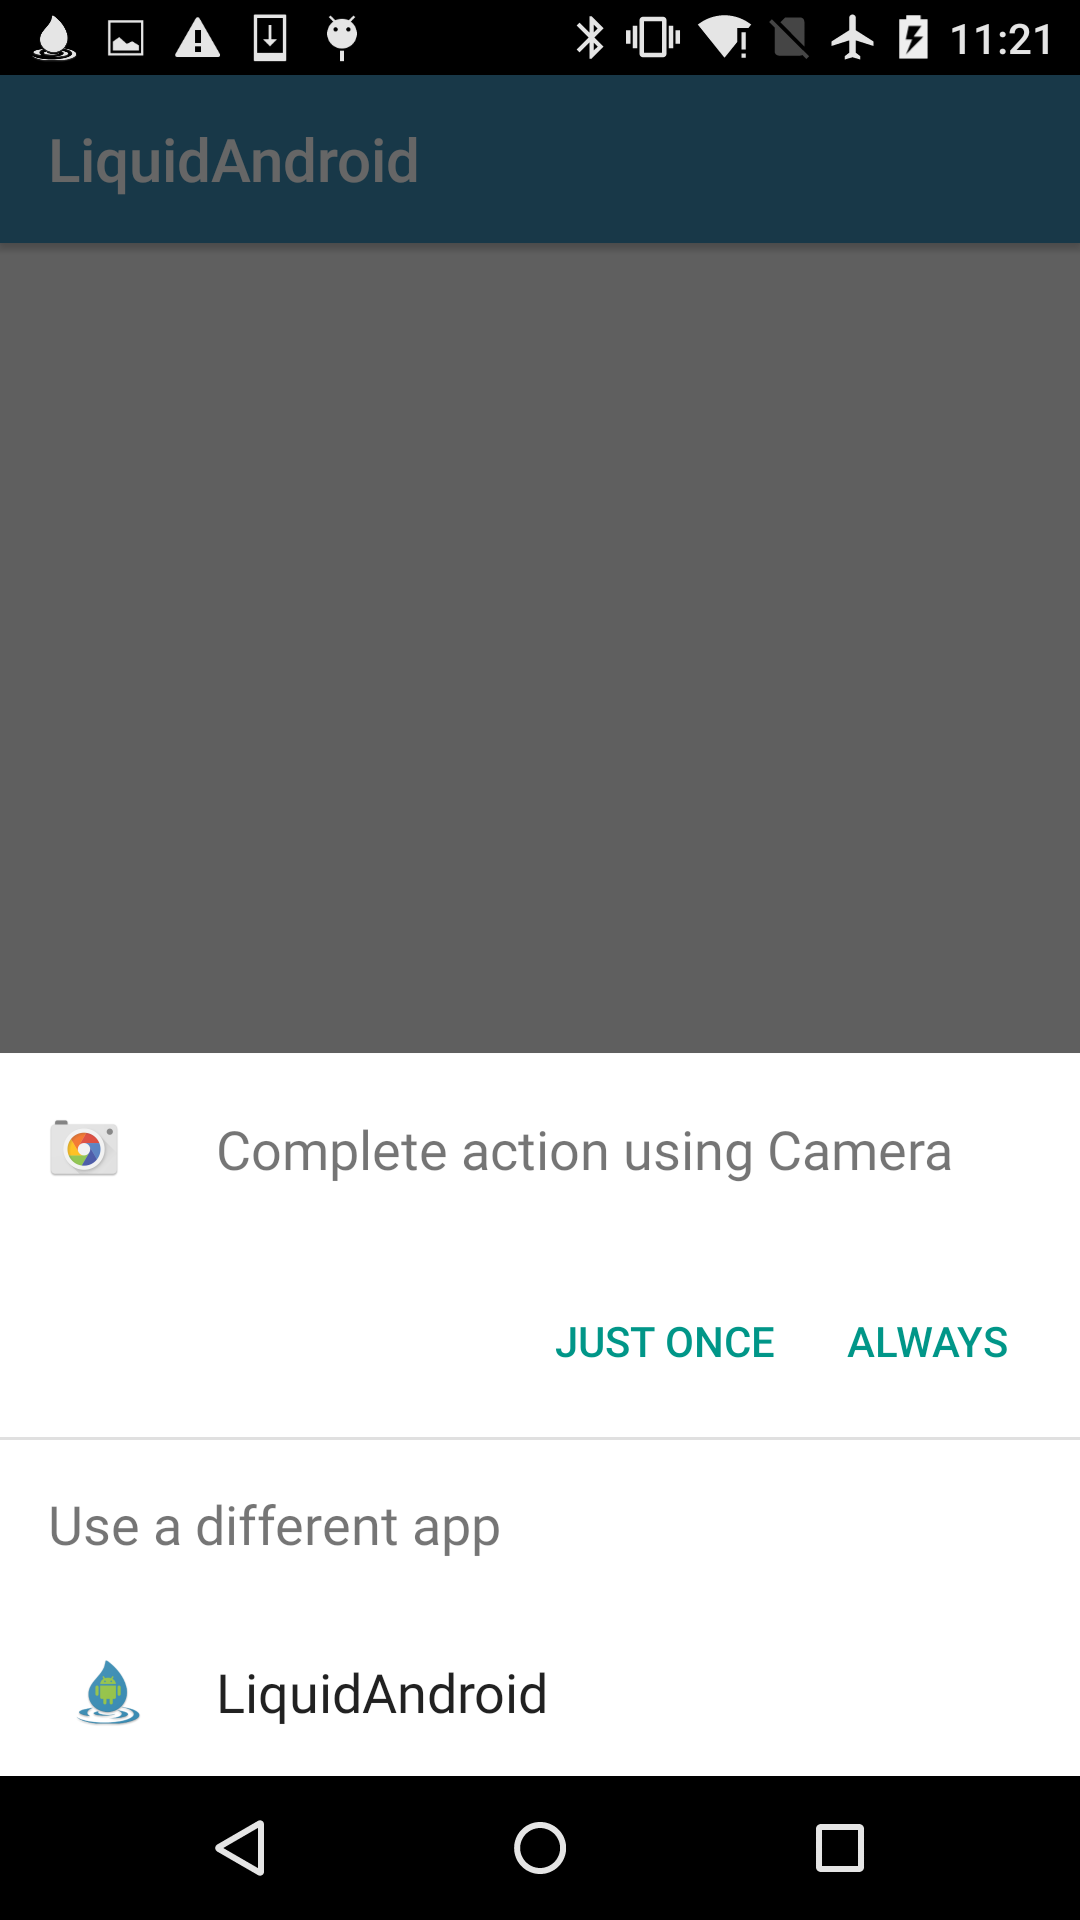
\includegraphics[width=0.9\textwidth]{chosephoto3}
		}
	\end{minipage}
	\begin{minipage}{.24\textwidth}\centering
		\bigskip
		\subfloat[Android Camera\label{subfig-7:camera2}]{%
			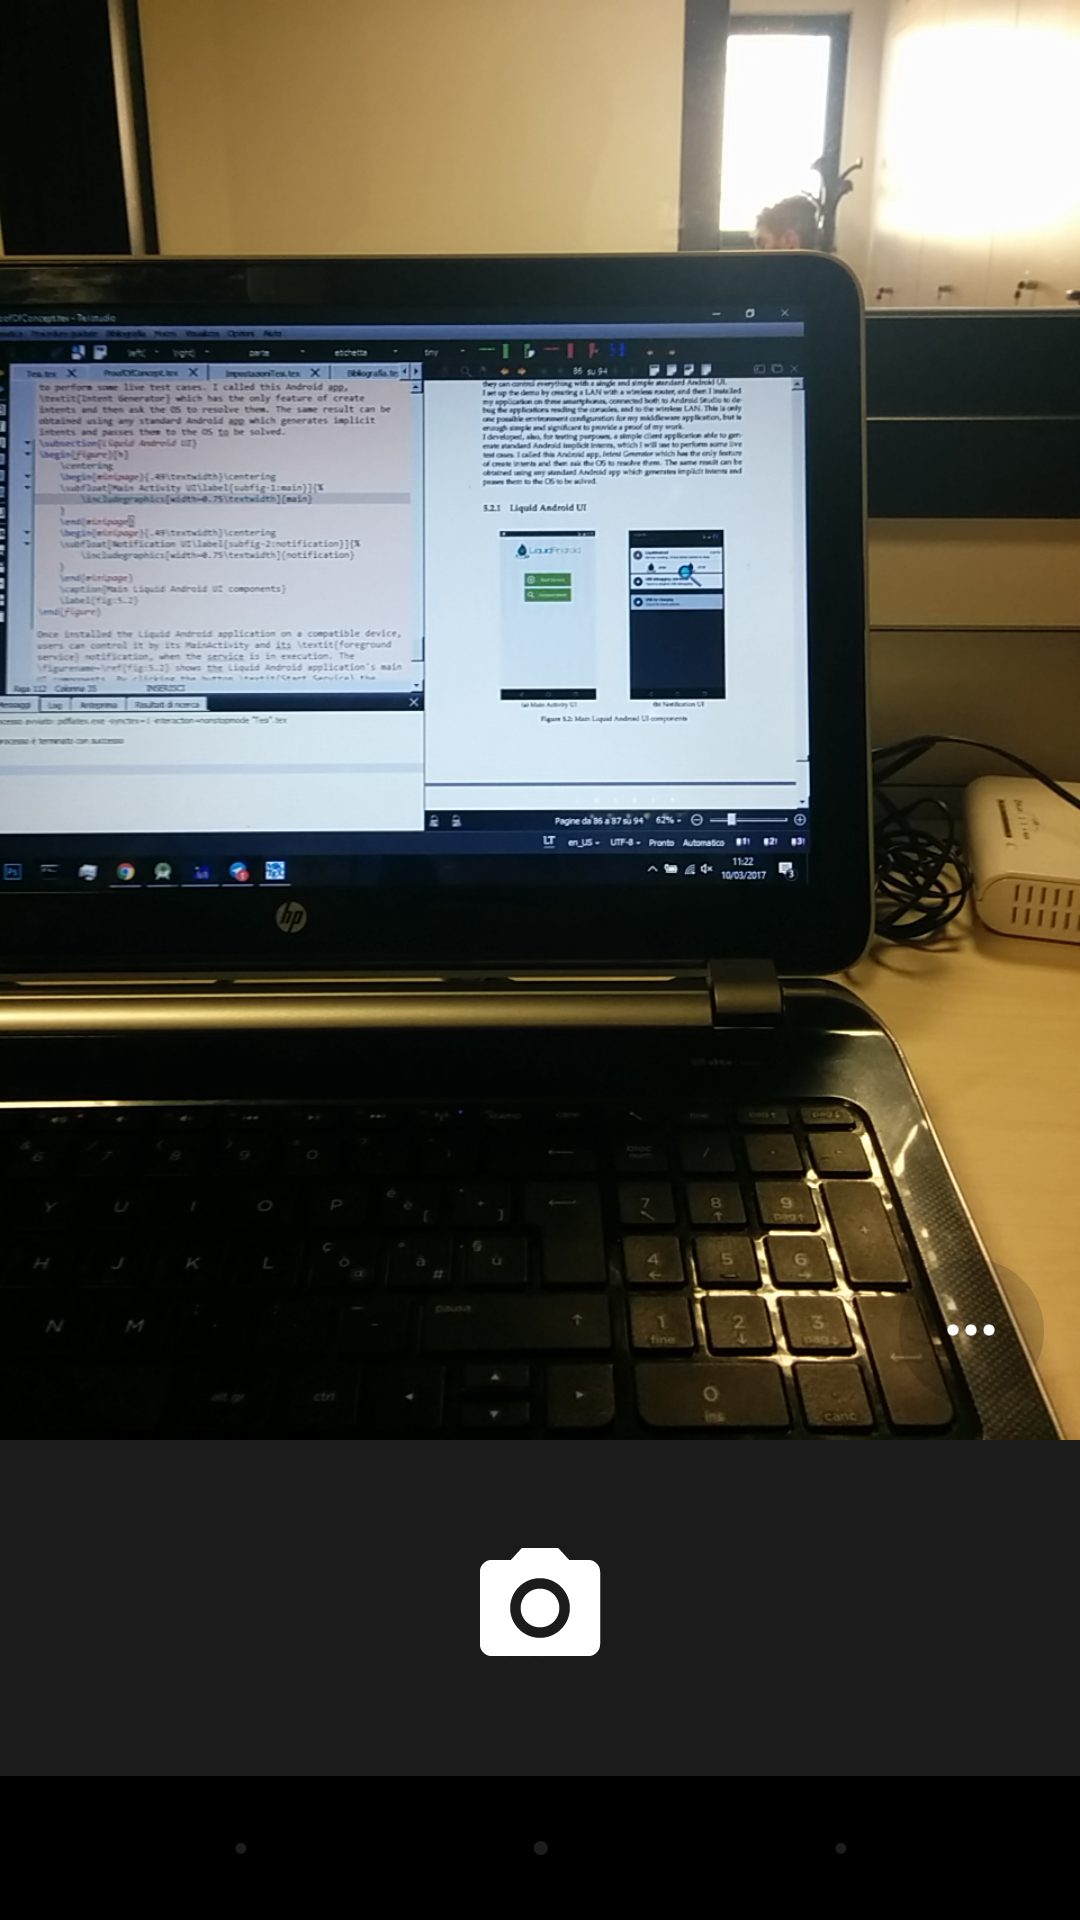
\includegraphics[width=0.9\textwidth]{camera1}
		}
	\end{minipage}
	\begin{minipage}{.24\textwidth}\centering
		\bigskip
		\subfloat[Result Activity\label{subfig-8:chooser2}]{%
			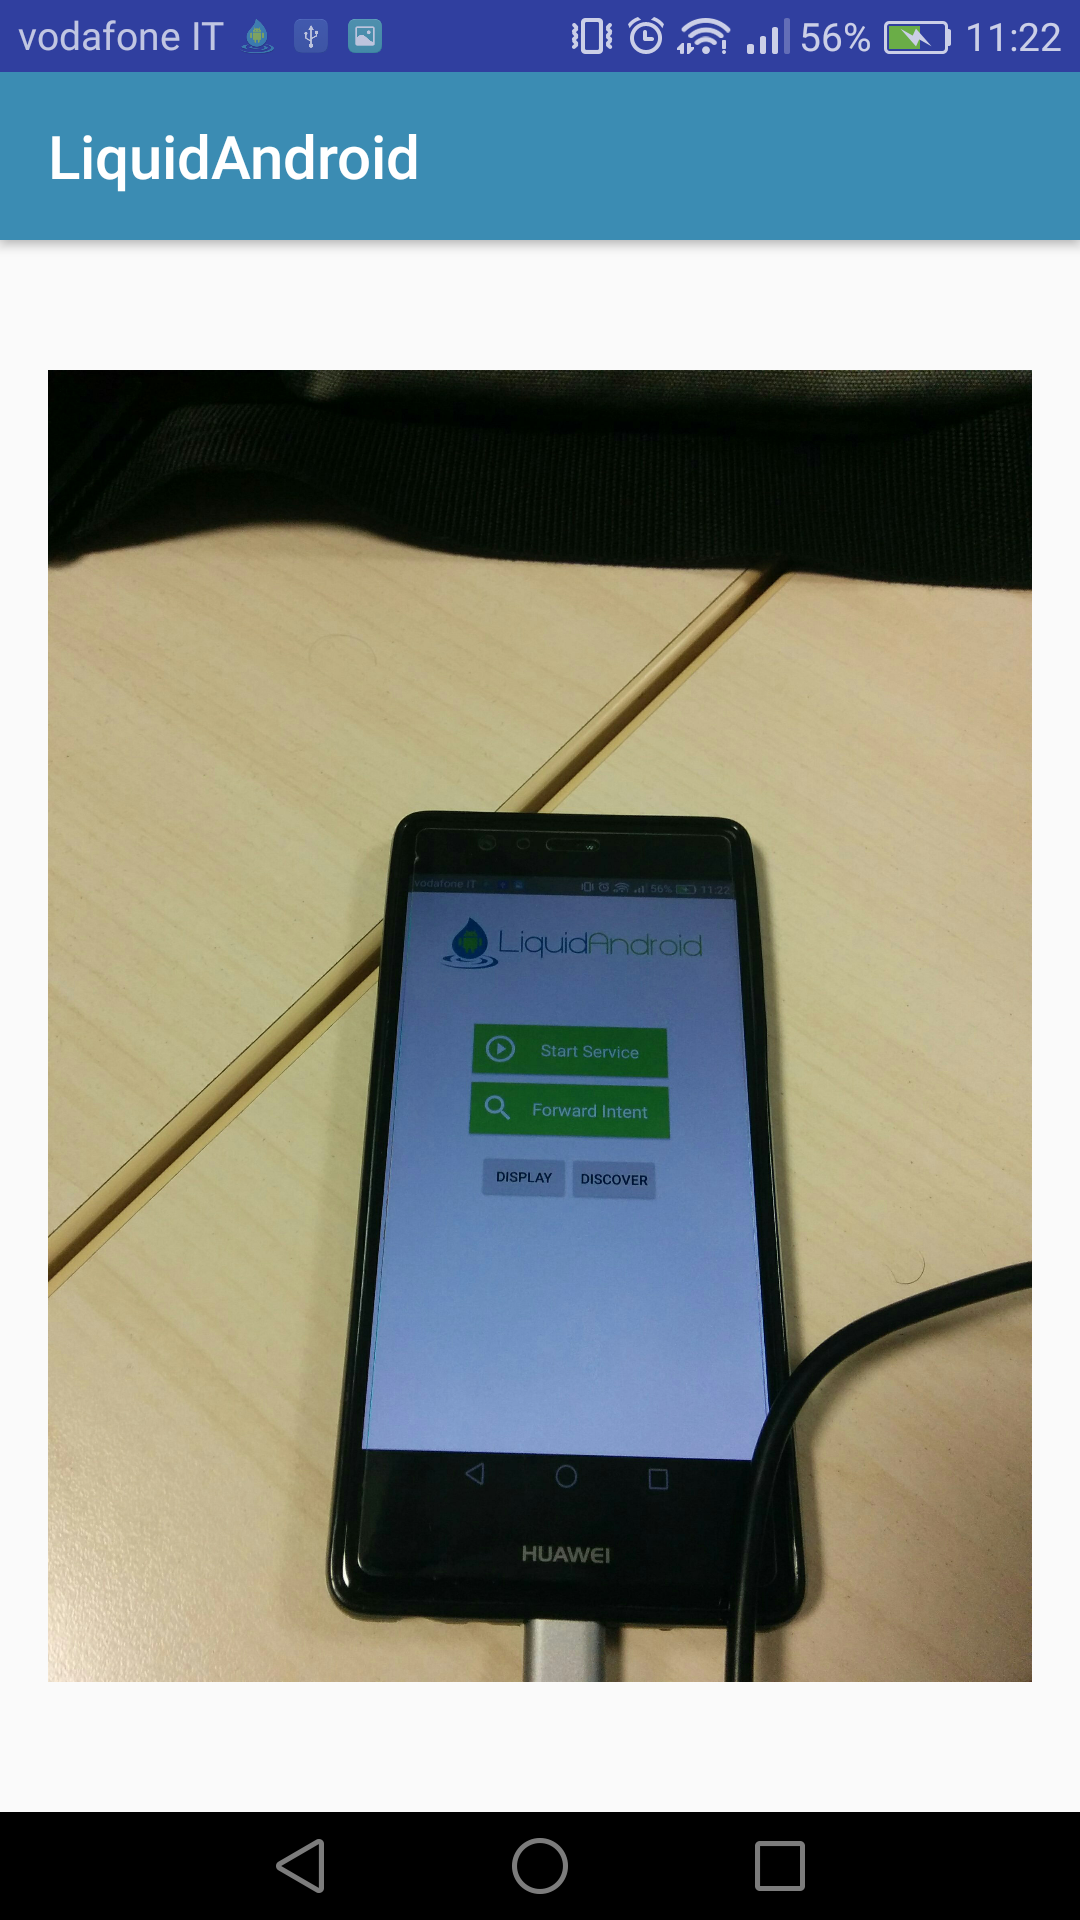
\includegraphics[width=0.9\textwidth]{received1}
		}
	\end{minipage}
	\caption{Complete photo intent live test screenshots}
	
\end{figure}\\
Screens \textit{d} and \textit{e} are taken from the first target device, a LG L70, used to take the first picture. Screens \textit{f} and \textit{g} are taken instead, from the second target device, a Google Nexus 5, used to take the second picture. In the end screen \textit{h} is taken again from the first device, showing the picture taken. All the pictures taken while performing this test, are saved locally on the local storage of the devices which have actually taken the picture, moreover they are saved in the local data storage of the caller device, and are accessible form its gallery application.

\section{Liquid Museum}
In this section I want to provide a real use of case for my framework, so I developed, for this purpose, two Android applications, using the Liquid Android API, which are a concrete example of how special purposes distributed applications can be easily and fast, built exploiting my solutions and my system.\\
The distributed application I have developed is composed of two APKs, one acting as a server app and one acting, indeed, as a client. These applications are supposed to be used in a real life use case: they aims to improve the experience of a guided tour in a museum. Both applications, are fully accessible on GitHub, the server app, \textit{Liquid Museum} at \href{https://github.com/mola15/LiquidMuseum}{github.com/mola15/LiquidMuseum}, and the client side app, \textit{Museum Client} at \href{https://github.com/mola15/MuseumClient}{github.com/mola15/MuseumClient}.
\subsection{System Structure}
\begin{figure}[h]
	\centering
	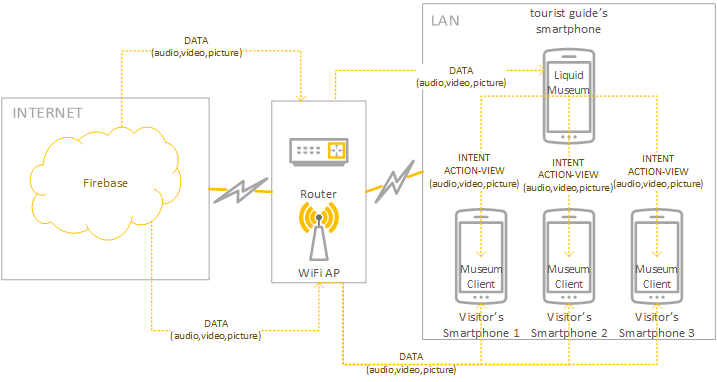
\includegraphics[width=1\textwidth]{museumstructure}
	\caption{Liquid Museum distributed structure}
	\label{fig:5.10}
\end{figure}
I developed the two applications using the mechanisms described in the previous sections of this work. I embedded the Liquid Android API structure, and I used it to let the server application spread intents, exploiting JSON-Intents, to all the devices having the client application installed and with the service already started. \figurename~\ref{fig:5.10} describes the complete structure of this application. In this case I decided to solve the data management problem with a cloud solution. Data, in fact, are stored in the cloud using the \textit{Firebase Platform}, by Google, which provides, among other things, a cloud storage, in which it is possible to easily save and manage any kind of file. The Liquid Museum application has been designed to be used by a tourist guide while he, or she, is doing his job, in a museum, during a guided tour with a group of tourist. The client app, Museum client, has been designed to be installed on the tourists' devices, to receive extra contents, in the form of distributed intents, while following their tourist guide in the museum guided tour. In this way the server applications works as a controller for the client one, and it can retrieve the right contents in the cloud and spread them to the clients, only by pressing some buttons in a control Activity. In this way the use of my distributed application enriches the guided tour providing insights, images, audios and video contents.
\subsection{Functionalities}
As I stated in the previous subsection, the client app can only connects to the server one to receive JSON-Intents, reconstruct the original Android intent and execute it. It contains only a simple UI to start the service, which is exactly the same of the Liquid Android API: it works in background and can be controlled with the very same notification I have described in \figurename~\ref{subfig-2:notification}. \\
To speed up the development and test phase of this application the two applications register their service using the same name \textit{Museum}, but in a real museum environment, in which different tourist guides performs different guided tours at the same time there is the need to let the user change this name, in order to connect only the desired devices to the tourist guide's Android device. To solve this problem it would be enough to record the various services by adding to the name, the \textit{ID} of the tourist guide.\\
The server app have a control interface activity, with which it is possible to send contents to all the clients in range only by pressing a button. In particular my application can send video, audio and picture contents and also web contents, such as \textit{URLs}. Furthermore the server application con play/pause the audio contents previously sent to the clients by using the audio controls button.\\
\begin{figure}[h]
	\centering
	\begin{minipage}{.49\textwidth}\centering
		\subfloat[Liquid Museum MainActivity\label{subfig-1:liquidmuseum}]{%
			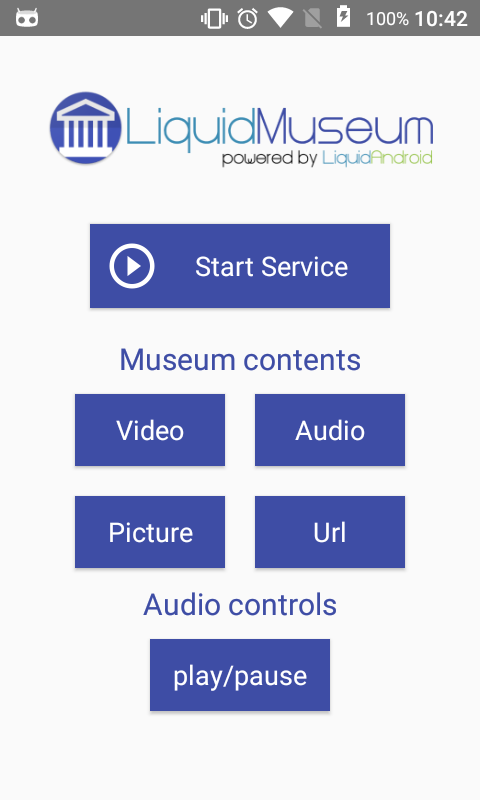
\includegraphics[width=0.75\textwidth]{liquidmuseum}
		}
	\end{minipage}
	\begin{minipage}{.49\textwidth}\centering
		\subfloat[Museum Client MainActivity\label{subfig-2:museumcclient}]{%
			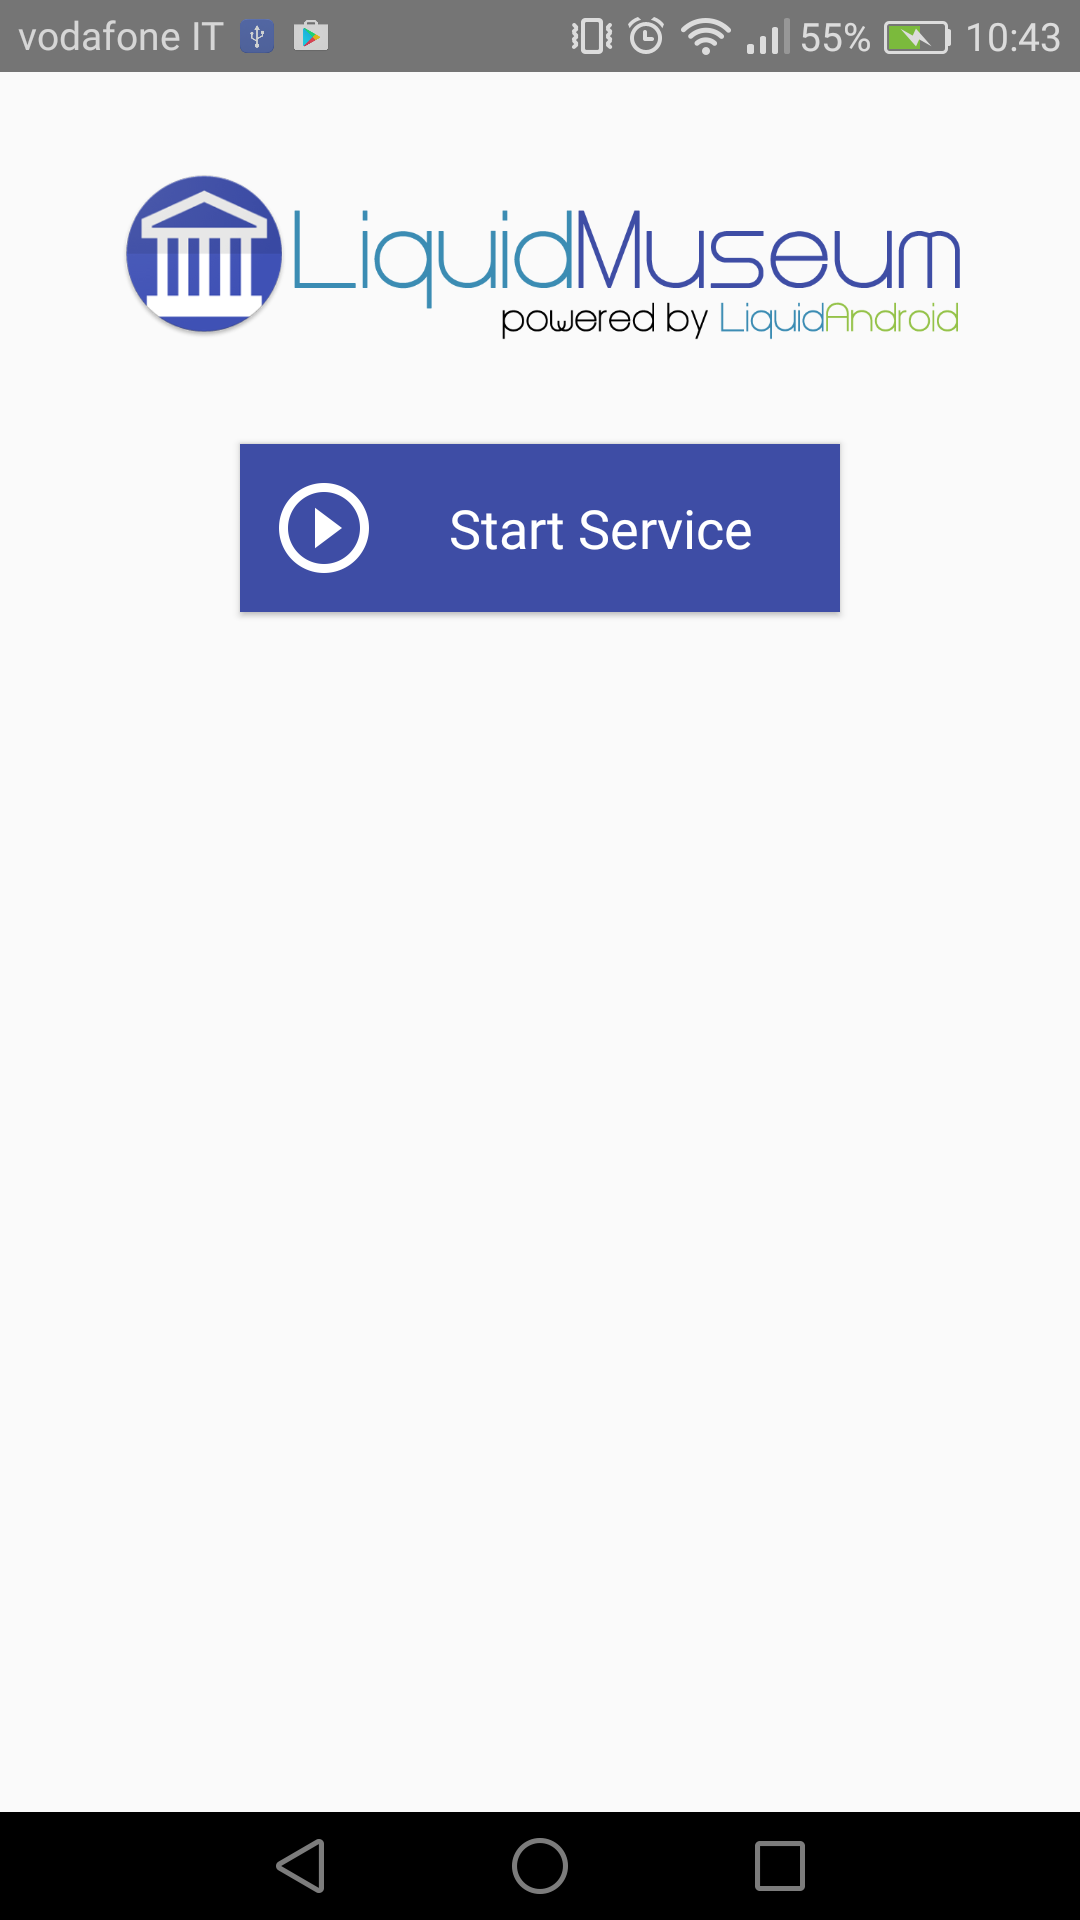
\includegraphics[width=0.75\textwidth]{museumclient}
		}
	\end{minipage}
	\caption{Liquid Museum and Museum Client UIs}
	\label{fig:5.11}
\end{figure}
\figurename~\ref{fig:5.11} shows the UIs for the two applications, in particular in \ref{subfig-1:liquidmuseum} there is the server application UI for \textit{Liquid Museum}, while in \ref{subfig-2:museumcclient} there is the client application UI for \textit{Museum Client}.
\subsection{Liquid Museum Live tests}

\bigskip
\par This section exhausts the topic, the next chapter deals with the conclusions which can be drawn from my thesis and any future work which can be done to extend and make the work as complete as possible.